\documentclass{slide}

\usepackage{changepage}
\usepackage{tabto}
\usepackage{tikz}
% \usepackage{pgfpages}
% \setbeameroption{show notes on second screen}

\title{Microservices Architecture}
\subtitle{Software Architecture}
\author{Richard Thomas}
\date{\week{8}}

\begin{document}

\maketitle

\begin{frame}{}
	\centering
	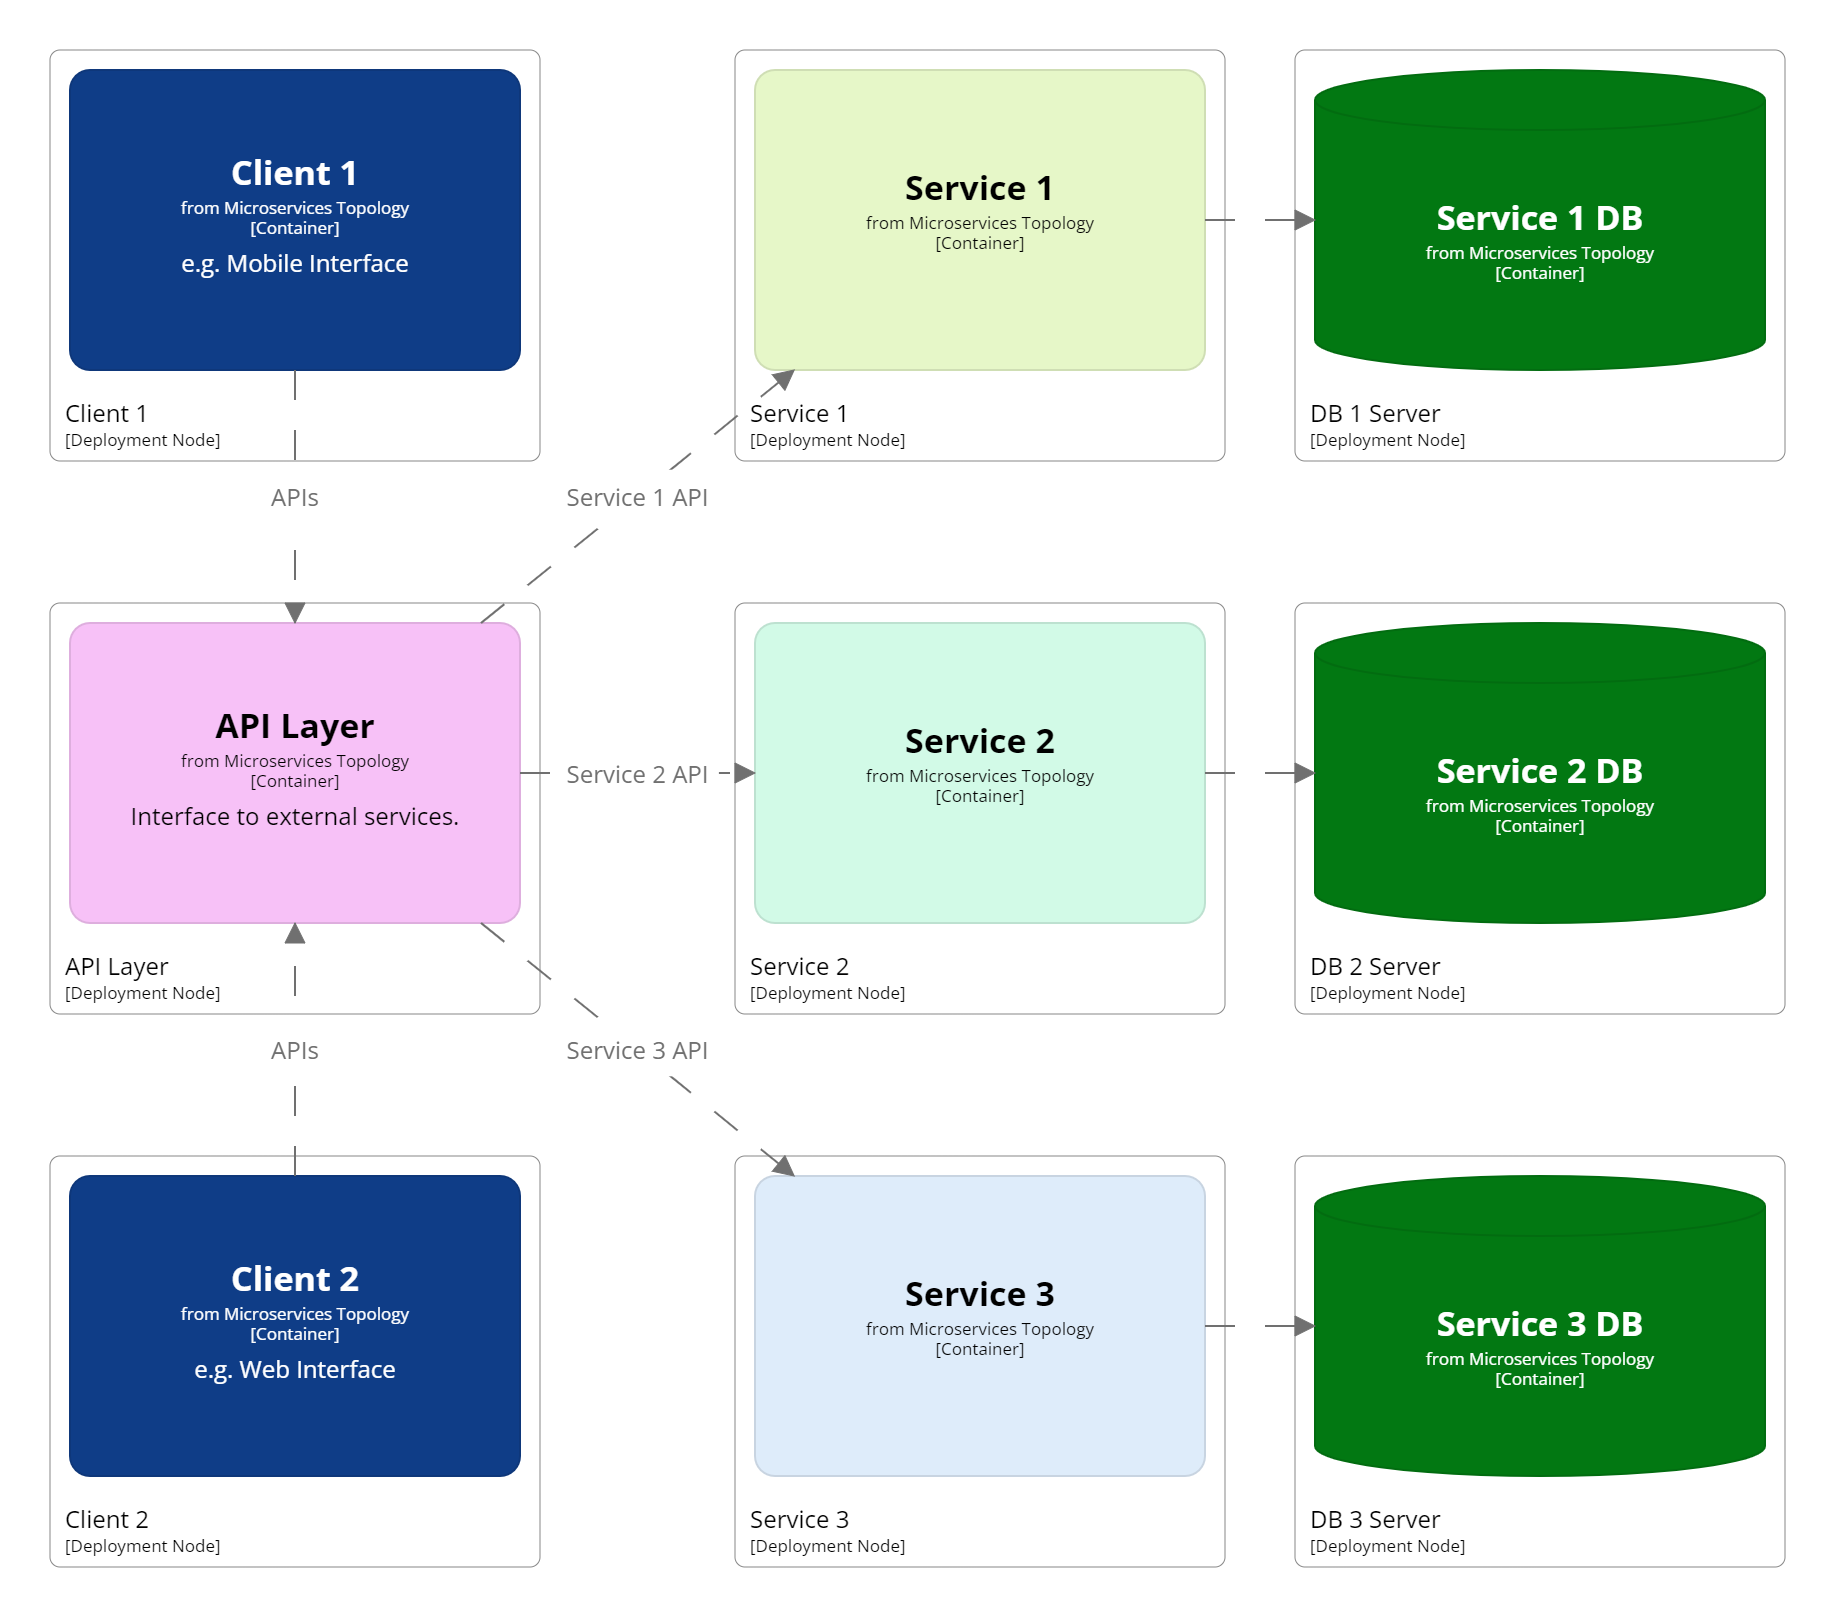
\includegraphics[trim=45 45 45 45,clip,height=\textheight]{diagrams/general-topology-deployment.png}
	\begin{tikzpicture}[overlay,remember picture]
	\node[rectangle,shift={(0.9,0.8)},
		  text width=7cm,above,rotate=90] at (current page.west) {\color{primary}\Large Microservices General Topology};
	\end{tikzpicture}   
\end{frame}
\note[itemize]{
    \item Multiple clients demonstrates common scenario of multiple interfaces to system (e.g. mobile, web).
    \item Client UIs may be monolithic to provide a rich interface.
}

\begin{frame}{API Layer Components}
    \centering
    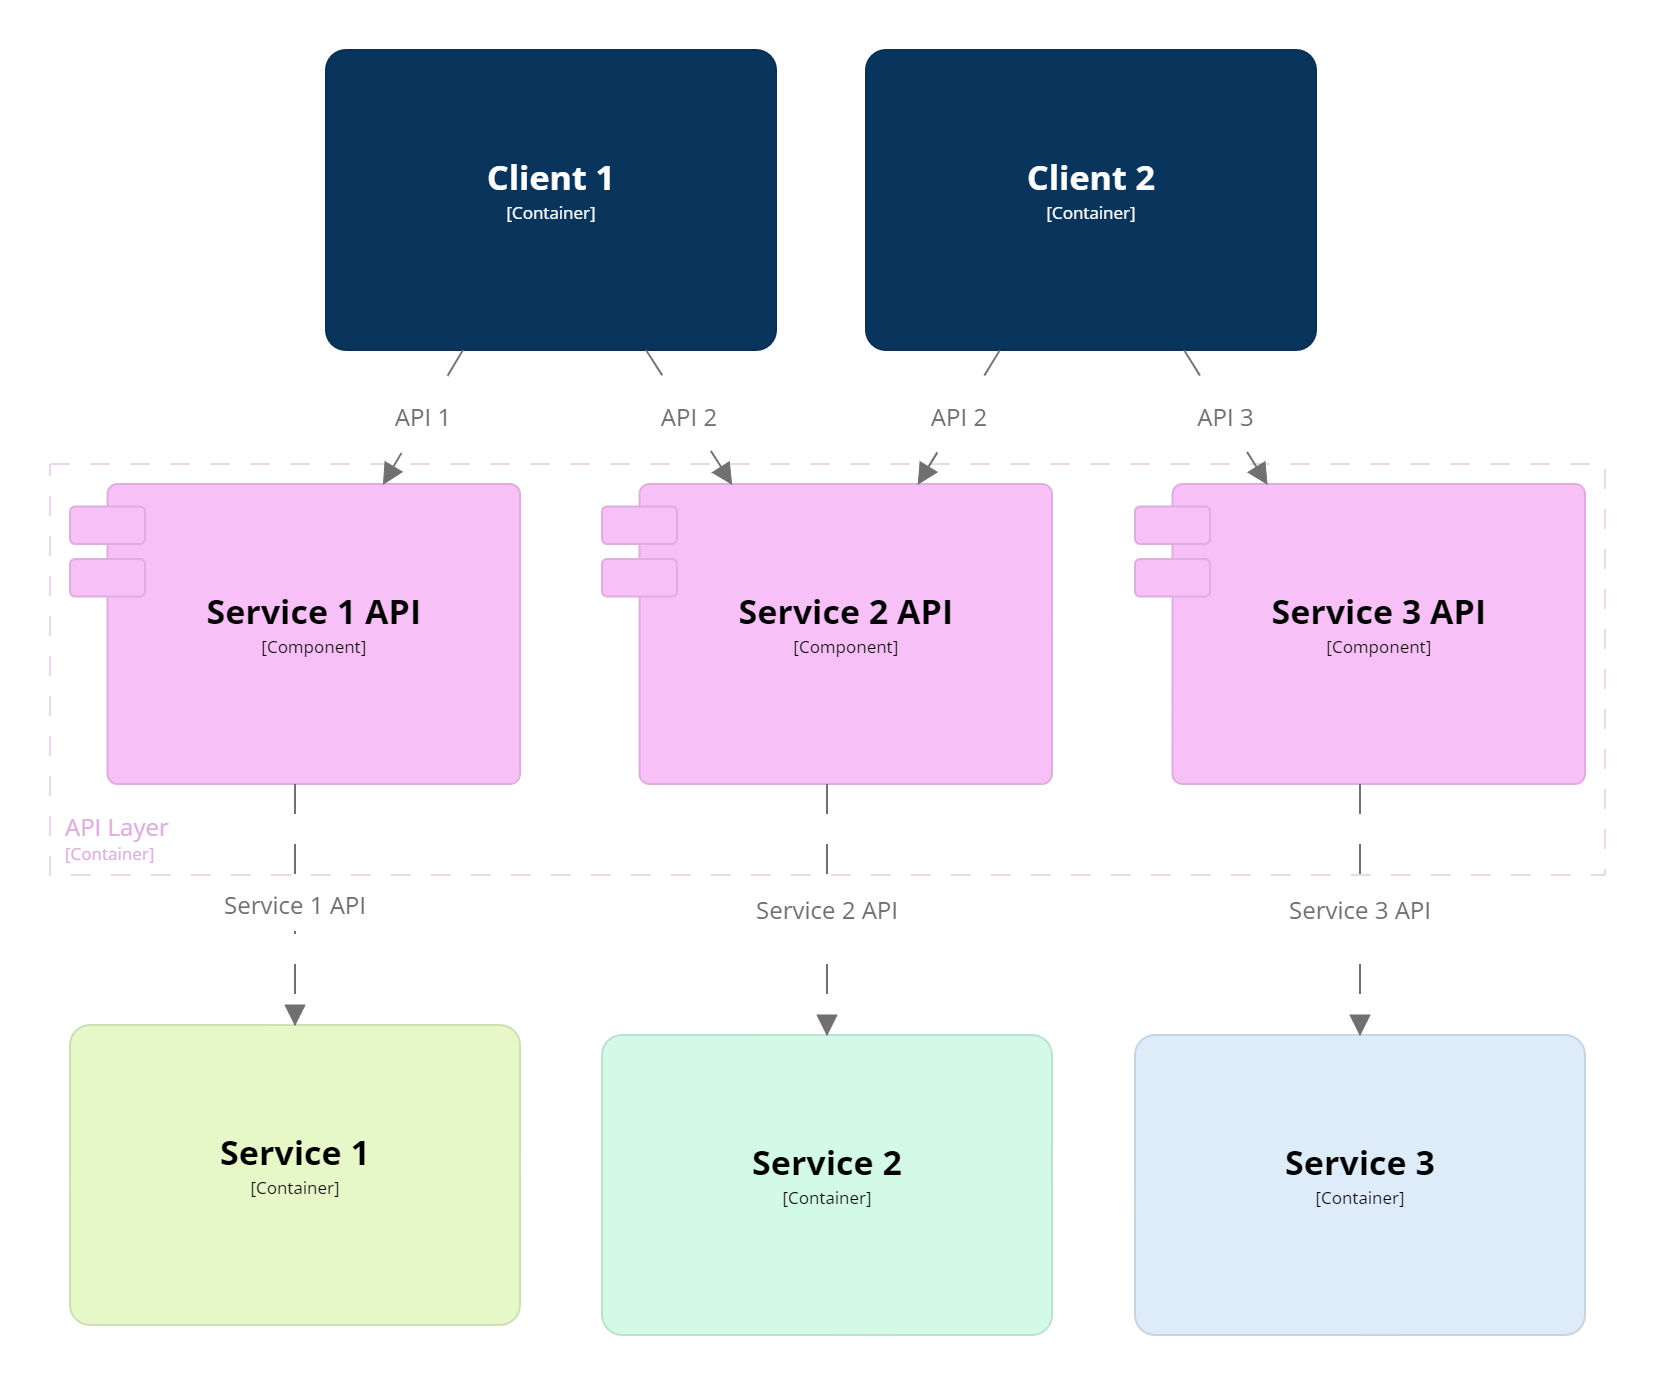
\includegraphics[trim=45 45 45 45,clip,width=0.9\textwidth]{diagrams/general-topology-api-component.png}
\end{frame}
\note[itemize]{
    \item Each client may use a different combination of services.
    \item API layer provides reverse proxy or gateway services, see Service-Based Architecture notes \& slides.
    \item Typically Service APIs in this layer have a one-to-one relationship with Services and are designed by the Service teams.
    \item Routing behaviour may not be required.
}

\begin{frame}{Service 1 Components}
    \begin{adjustwidth}{-10.5mm}{-10mm}
        \centering
        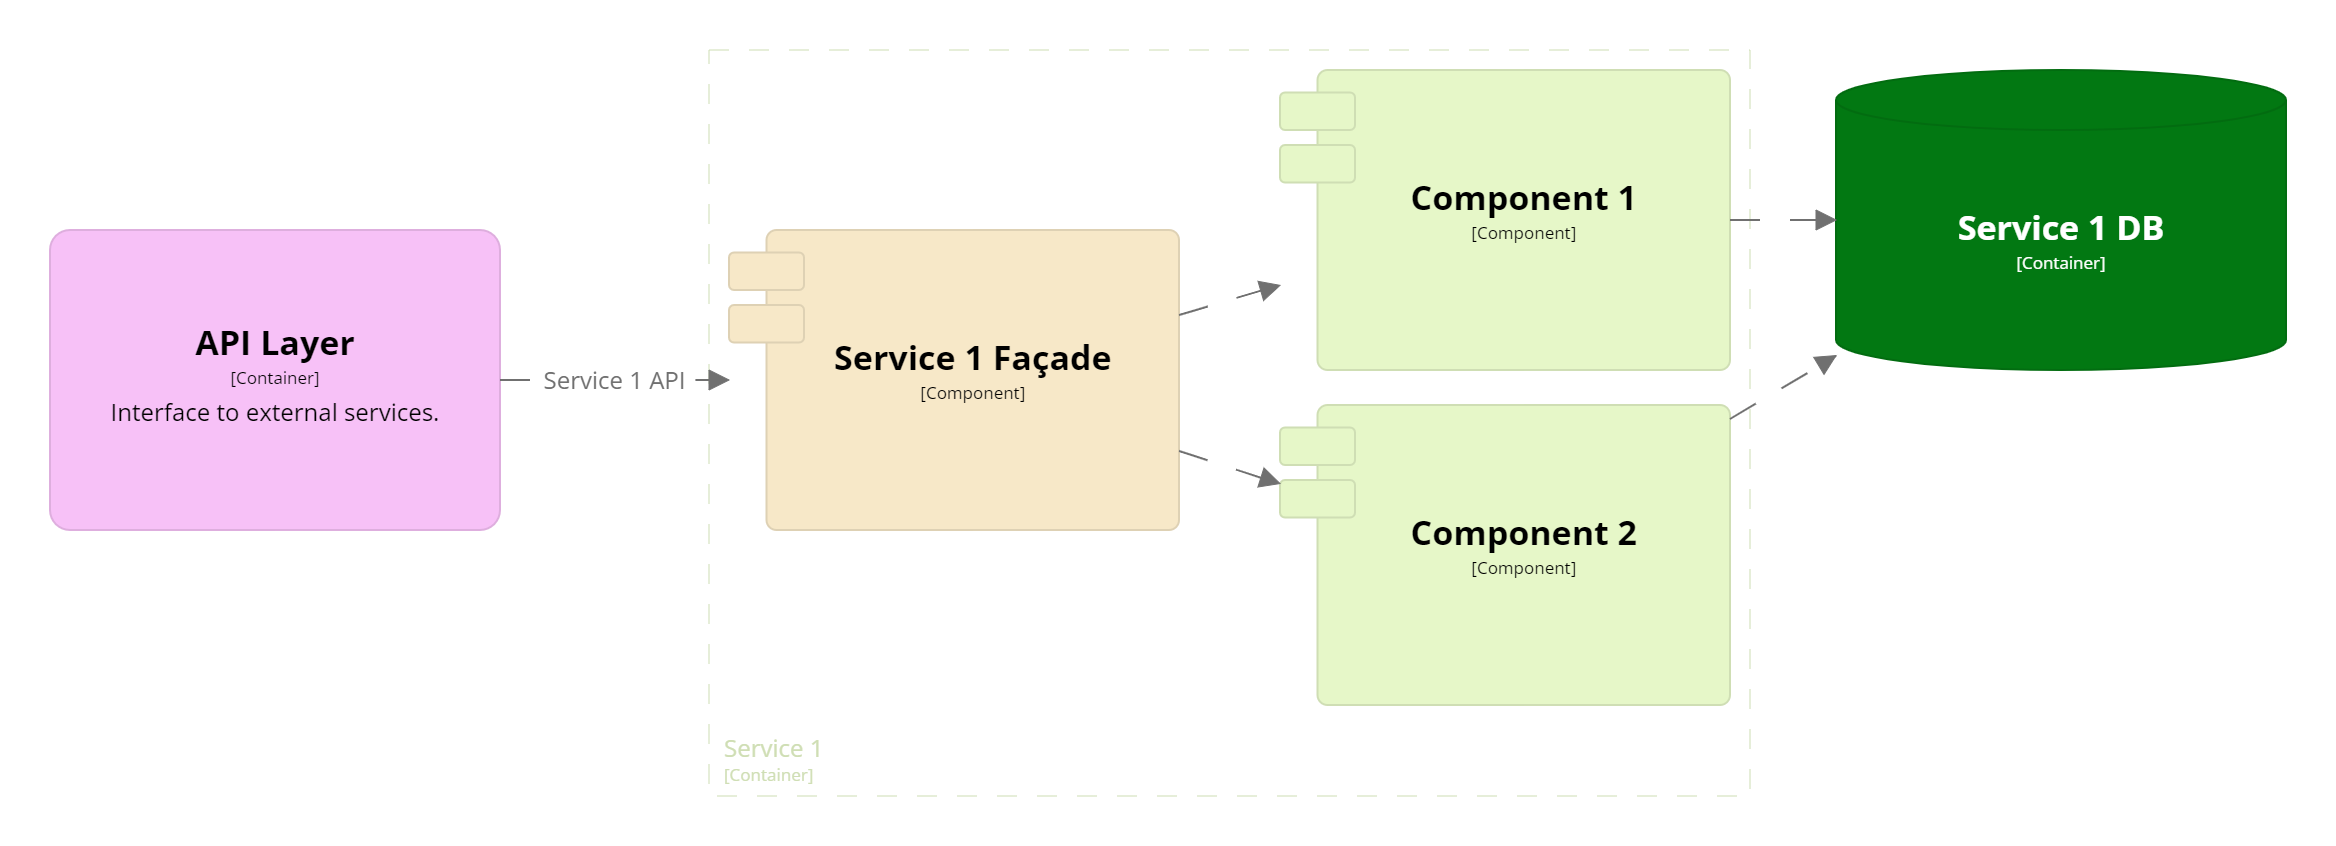
\includegraphics[trim=45 45 45 45,clip,width=0.99\paperwidth]{diagrams/general-topology-service1-component.png}
    \end{adjustwidth}
\end{frame}
\note{Services 2 \& 3 are essentially the same.}

\begin{frame}{Client with Monolithic UI}
    \centering
    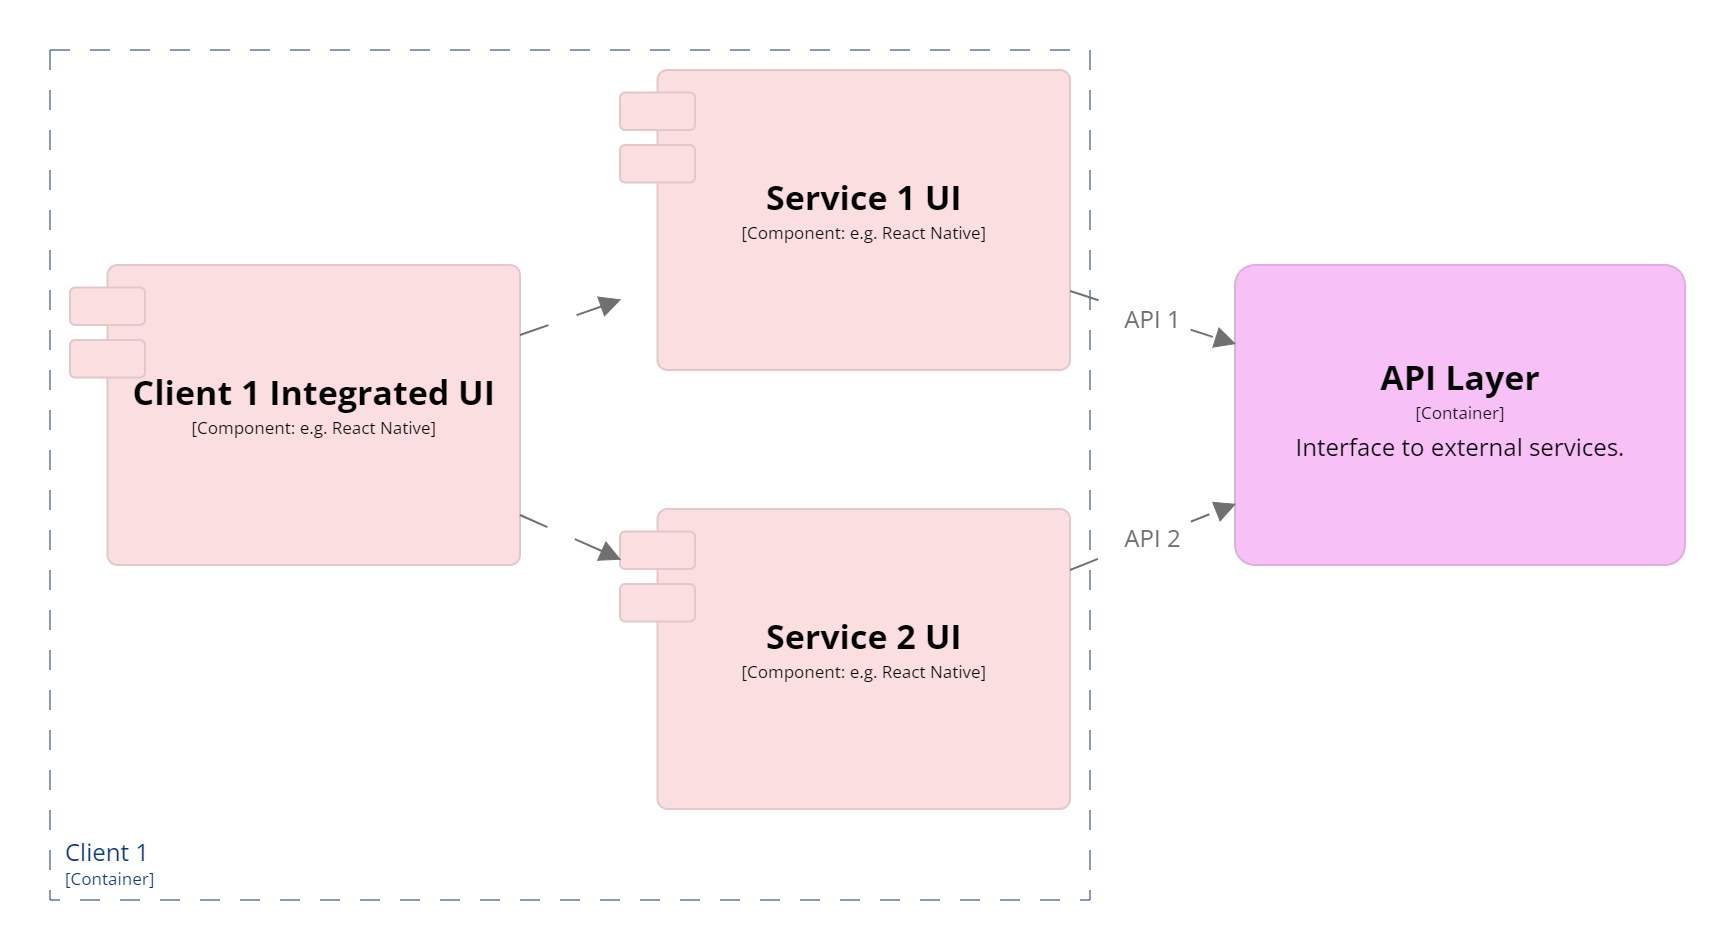
\includegraphics[trim=45 45 45 45,clip,width=0.9\textwidth]{diagrams/monolithic-ui-client1-component.png}
\end{frame}
\note[itemize]{
    \item Purist Microservices architecture -- each service development team builds their service's UI(s).
    \item Typically needs some coordinating activity in the UI.
    \item Can still have multiple UIs (e.g. web, mobile, ...).
}

\point[DDD Influence]{%
Services are \highlight{bounded contexts}.

Bounded contexts are not necessarily \highlight{services}.
}

\definition{Bounded Context}{Logical boundary of a domain where particular terms and rules apply consistently.}

\begin{frame}{}
	\centering
	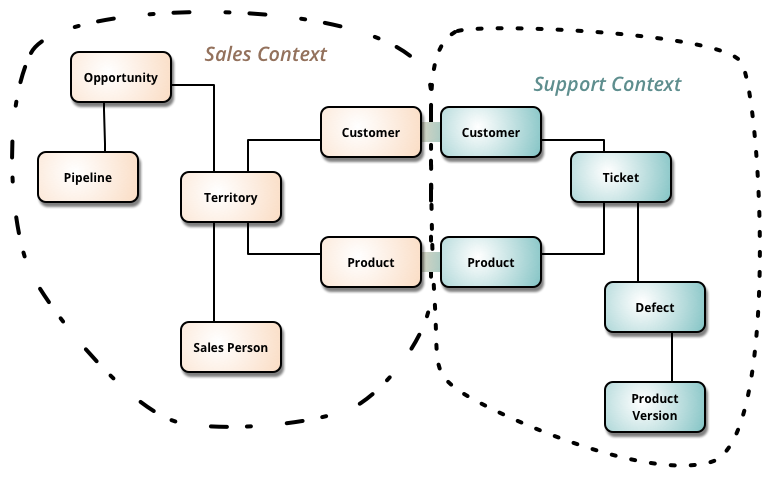
\includegraphics[height=.97\textheight]{diagrams/bounded-context.png}
	\begin{tikzpicture}[overlay,remember picture]
	\node[rectangle,shift={(-4.6,0)},
		  text width=6.5cm,above] at (current page.south) {\color{primary}\tiny From \url{https://martinfowler.com/bliki/BoundedContext.html}};
	\end{tikzpicture}   
\end{frame}

\definition{Service Cohesion Principle}{
Services are cohesive business processes.

They are a bounded context.
}

\begin{frame}{Large Bounded Contexts}
\LARGE
A bounded context may be too large to be a single service.
\\~\\
Split it into services that are \highlight{independent} sub-processes.
\end{frame}

\definition{Service Independence Principle}{Services should not depend on the implementation of other services.}

\corollary{Low Coupling}{There should be minimal coupling between services.}

\corollary{No Reuse}{
Avoid dependencies between services.

Do not reuse components between services.
}

\begin{frame}{Bounded Domains Implications}
    \LARGE
    \begin{itemize}
		\item<1-> Duplication
	    \begin{itemize}
	    		\vspace{2mm}
			\Large\item Entities specialised for domain
		    \begin{itemize}
				\large\item Requires mapping of entity data between domains
		    \end{itemize}
	    		\vspace{2mm}
			\Large\item<2-> Should everything be duplicated?
		    \begin{itemize}
				\large\item<3-> What about common services (e.g. logging, ...)?
		    \end{itemize}
	    \end{itemize}
	    \vspace{3mm}
		\item<4-> Heterogeneity
		\begin{itemize}
	    		\vspace{1mm}
			\Large\item Services can use different implementation technologies
		\end{itemize}
    \end{itemize}
\end{frame}

\begin{frame}{Service Plane}
	\centering
	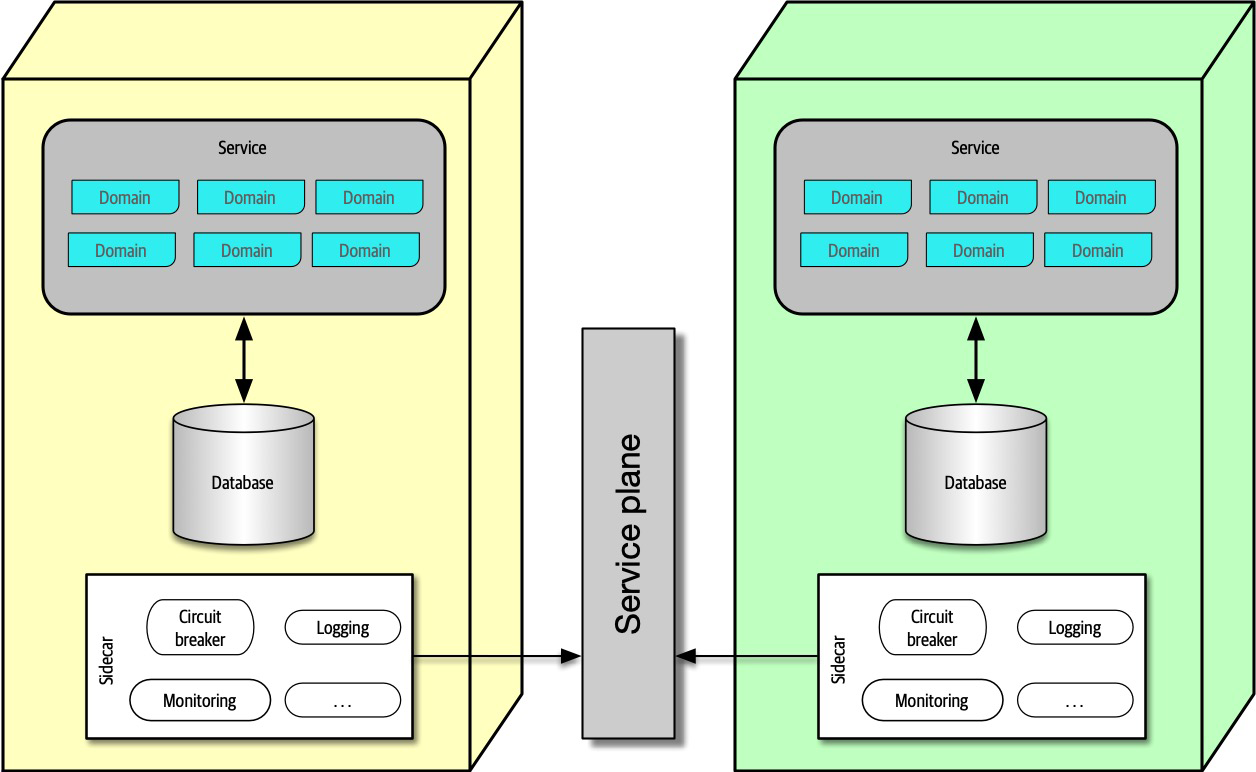
\includegraphics[height=.75\textheight]{diagrams/service-plane-sidecar.png}
	\begin{tikzpicture}[overlay,remember picture]
	\node[rectangle,shift={(-4.6,0)},
		  text width=6.5cm,above] at (current page.south) {\color{primary}\tiny From \textit{Fundamentals of Software Architecture}};
	\end{tikzpicture}   
\end{frame}

\begin{frame}{Service Mesh}
	\centering
	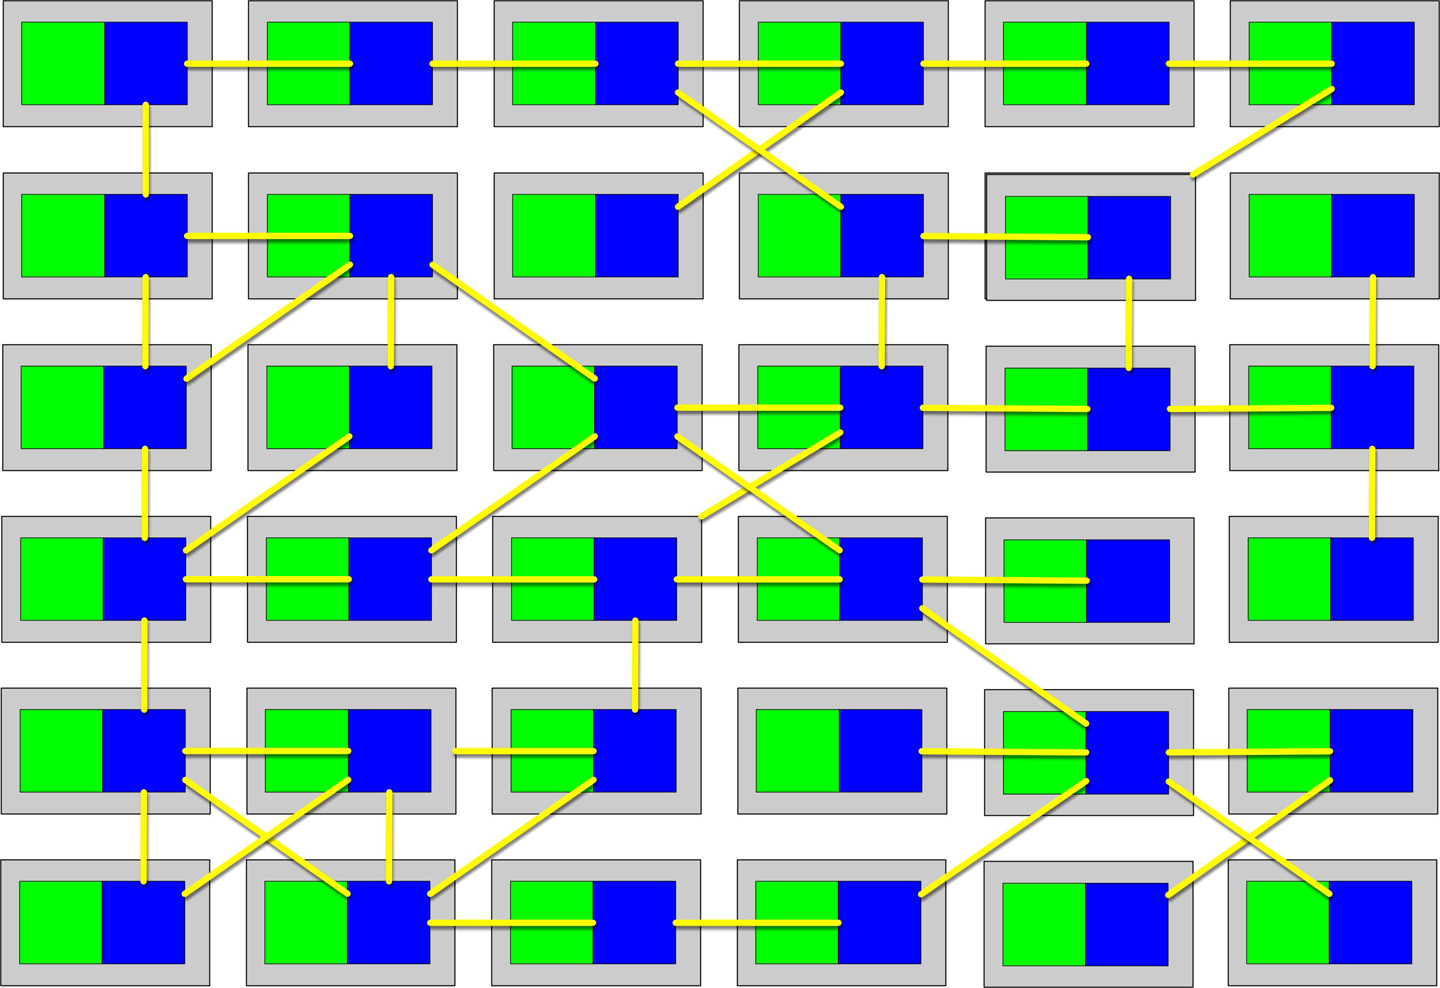
\includegraphics[height=.85\textheight]{diagrams/service-mesh.png}
	\begin{tikzpicture}[overlay,remember picture]
	\node[rectangle,shift={(-4.6,-0.1)},
		  text width=6.5cm,above] at (current page.south) {\color{primary}\tiny From \textit{Fundamentals of Software Architecture}};
	\end{tikzpicture}   
\end{frame}

{
\usebackgroundtemplate{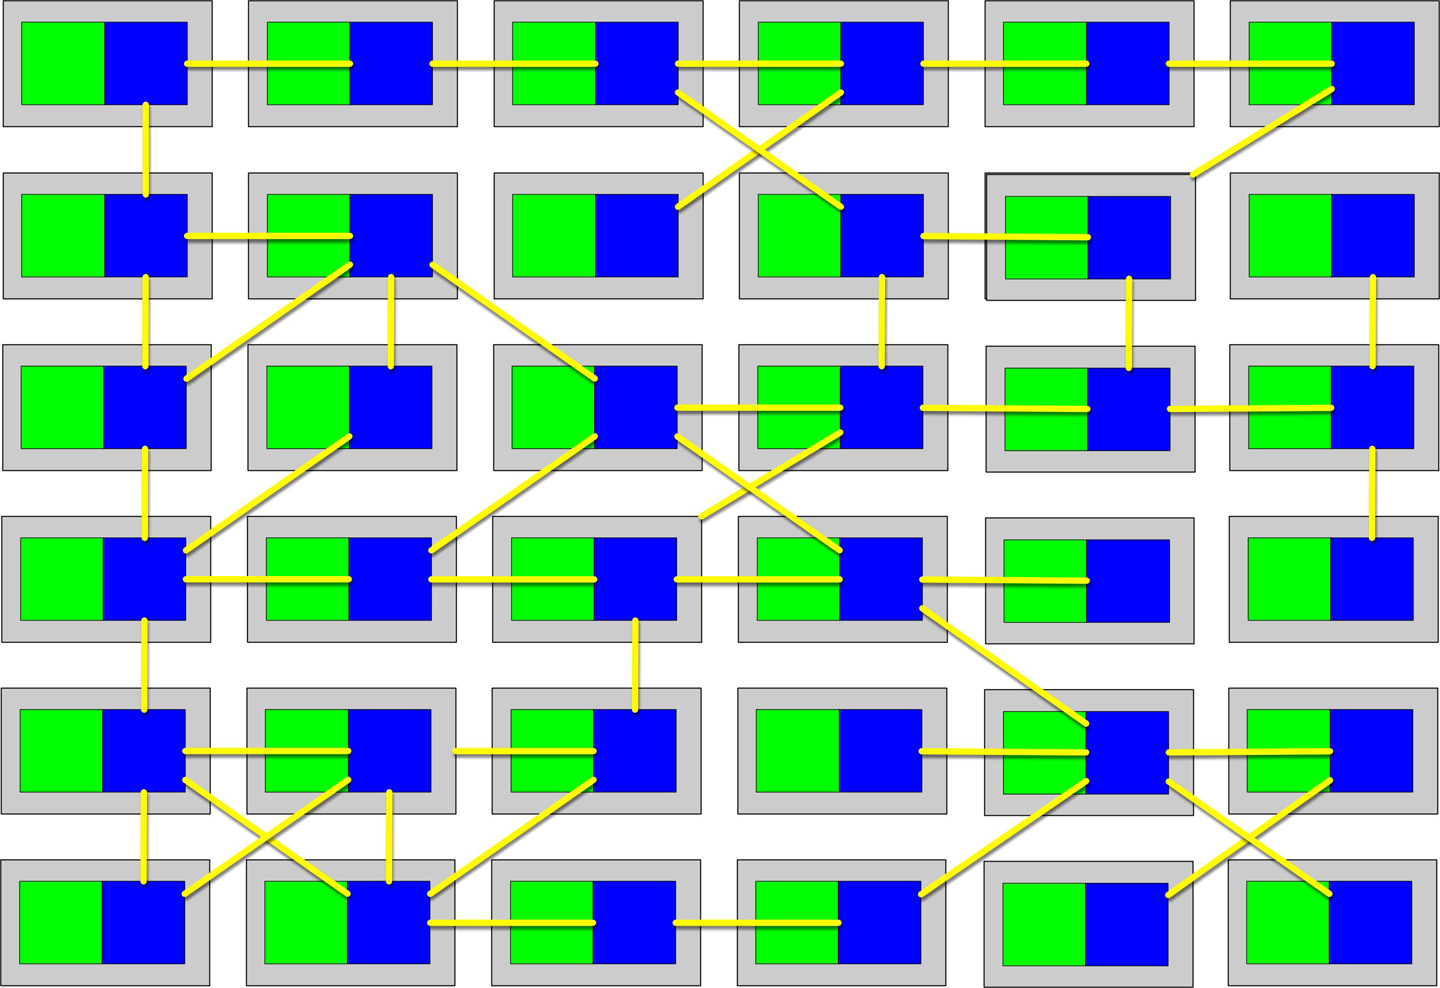
\includegraphics[trim=-80 0 0 -35,clip,height=0.95\paperheight]{diagrams/service-mesh.png}}
\begin{frame}{Service Mesh}
	\centering
	
\includegraphics[height=.65\textheight]{../../shared/images/fear.png}
	\begin{tikzpicture}[overlay,remember picture]
	\node[rectangle,shift={(-4.6,-0.1)},
		  text width=6.5cm,above] at (current page.south) {\color{primary}\tiny From \textit{Fundamentals of Software Architecture}};
	\end{tikzpicture}   
\end{frame}
}

\point[Choreography \& Orchestration]{
\begin{description}
    \item[Choreography] Similar to event-driven \highlight{broker}
    \item[Orchestration] Similar to event-driven \highlight{mediator}
\end{description}
}

\begin{frame}
    \begin{adjustwidth}{-10mm}{-10mm}
        \centering
        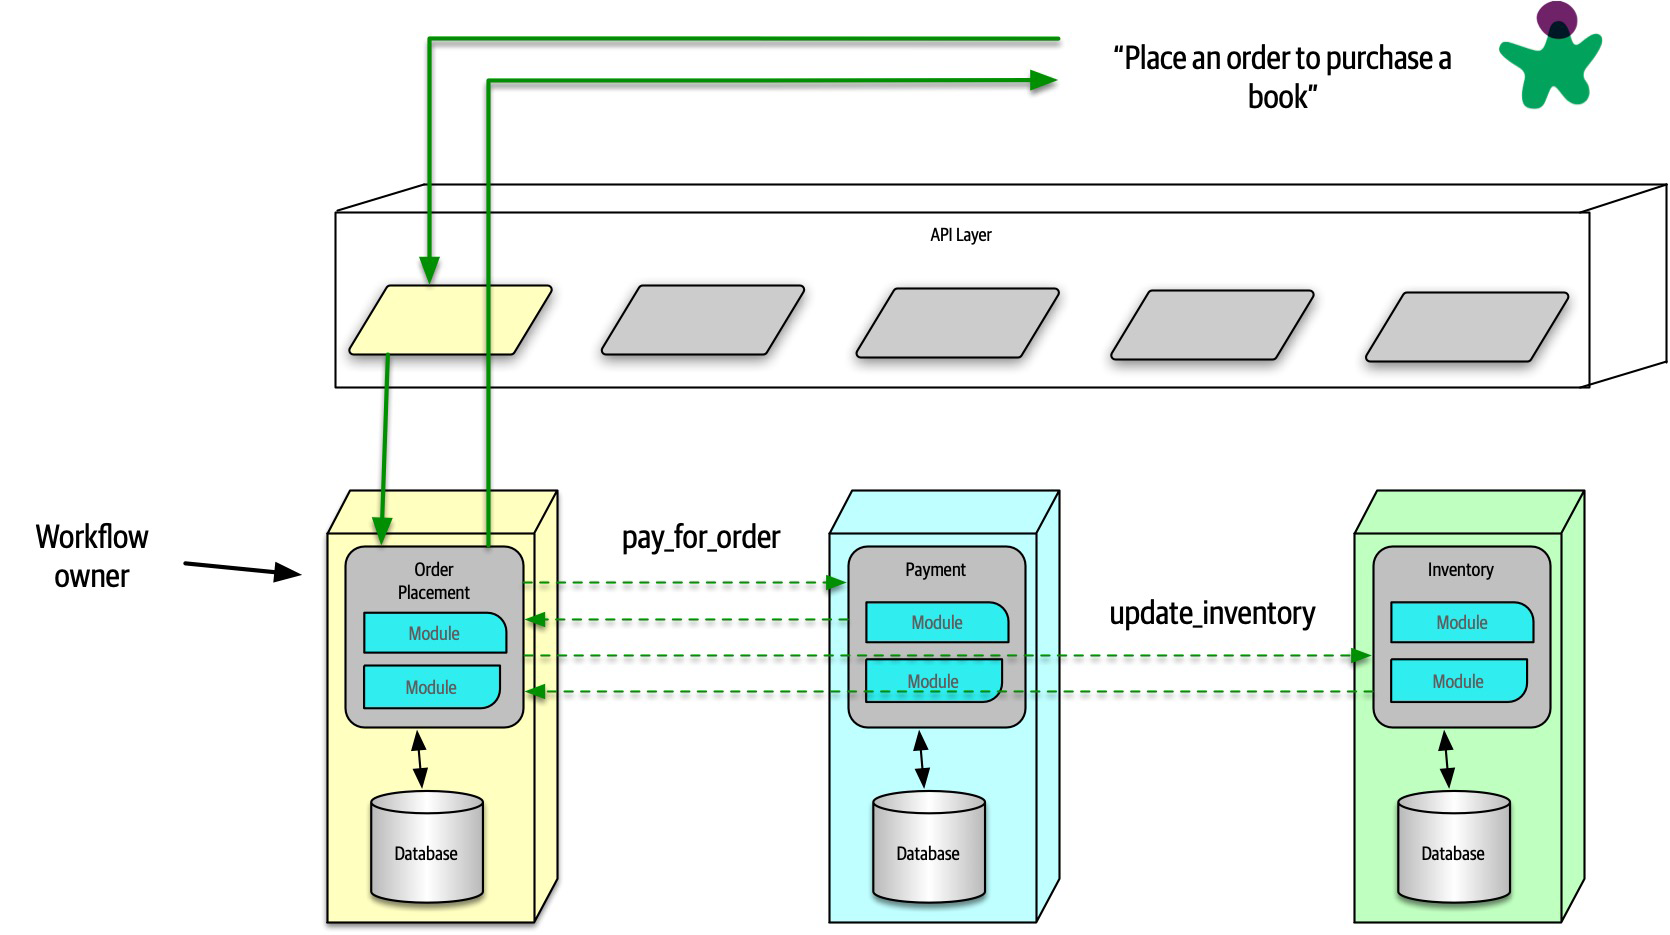
\includegraphics[width=0.96\paperwidth]{diagrams/choreography.png}
    \end{adjustwidth}
	\begin{tikzpicture}[overlay,remember picture]
	\node[rectangle,shift={(1.7,3.6)},
		  text width=3cm,above] at (current page.west) {\color{primary}\Large Choreography};
	\end{tikzpicture}   
	\begin{tikzpicture}[overlay,remember picture]
	\node[rectangle,shift={(-4.7,-0.1)},
		  text width=6.5cm,above] at (current page.south) {\color{primary}\tiny From \textit{Fundamentals of Software Architecture}};
	\end{tikzpicture}   
\end{frame}

\begin{frame}
    \begin{adjustwidth}{-10mm}{-10mm}
        \centering
        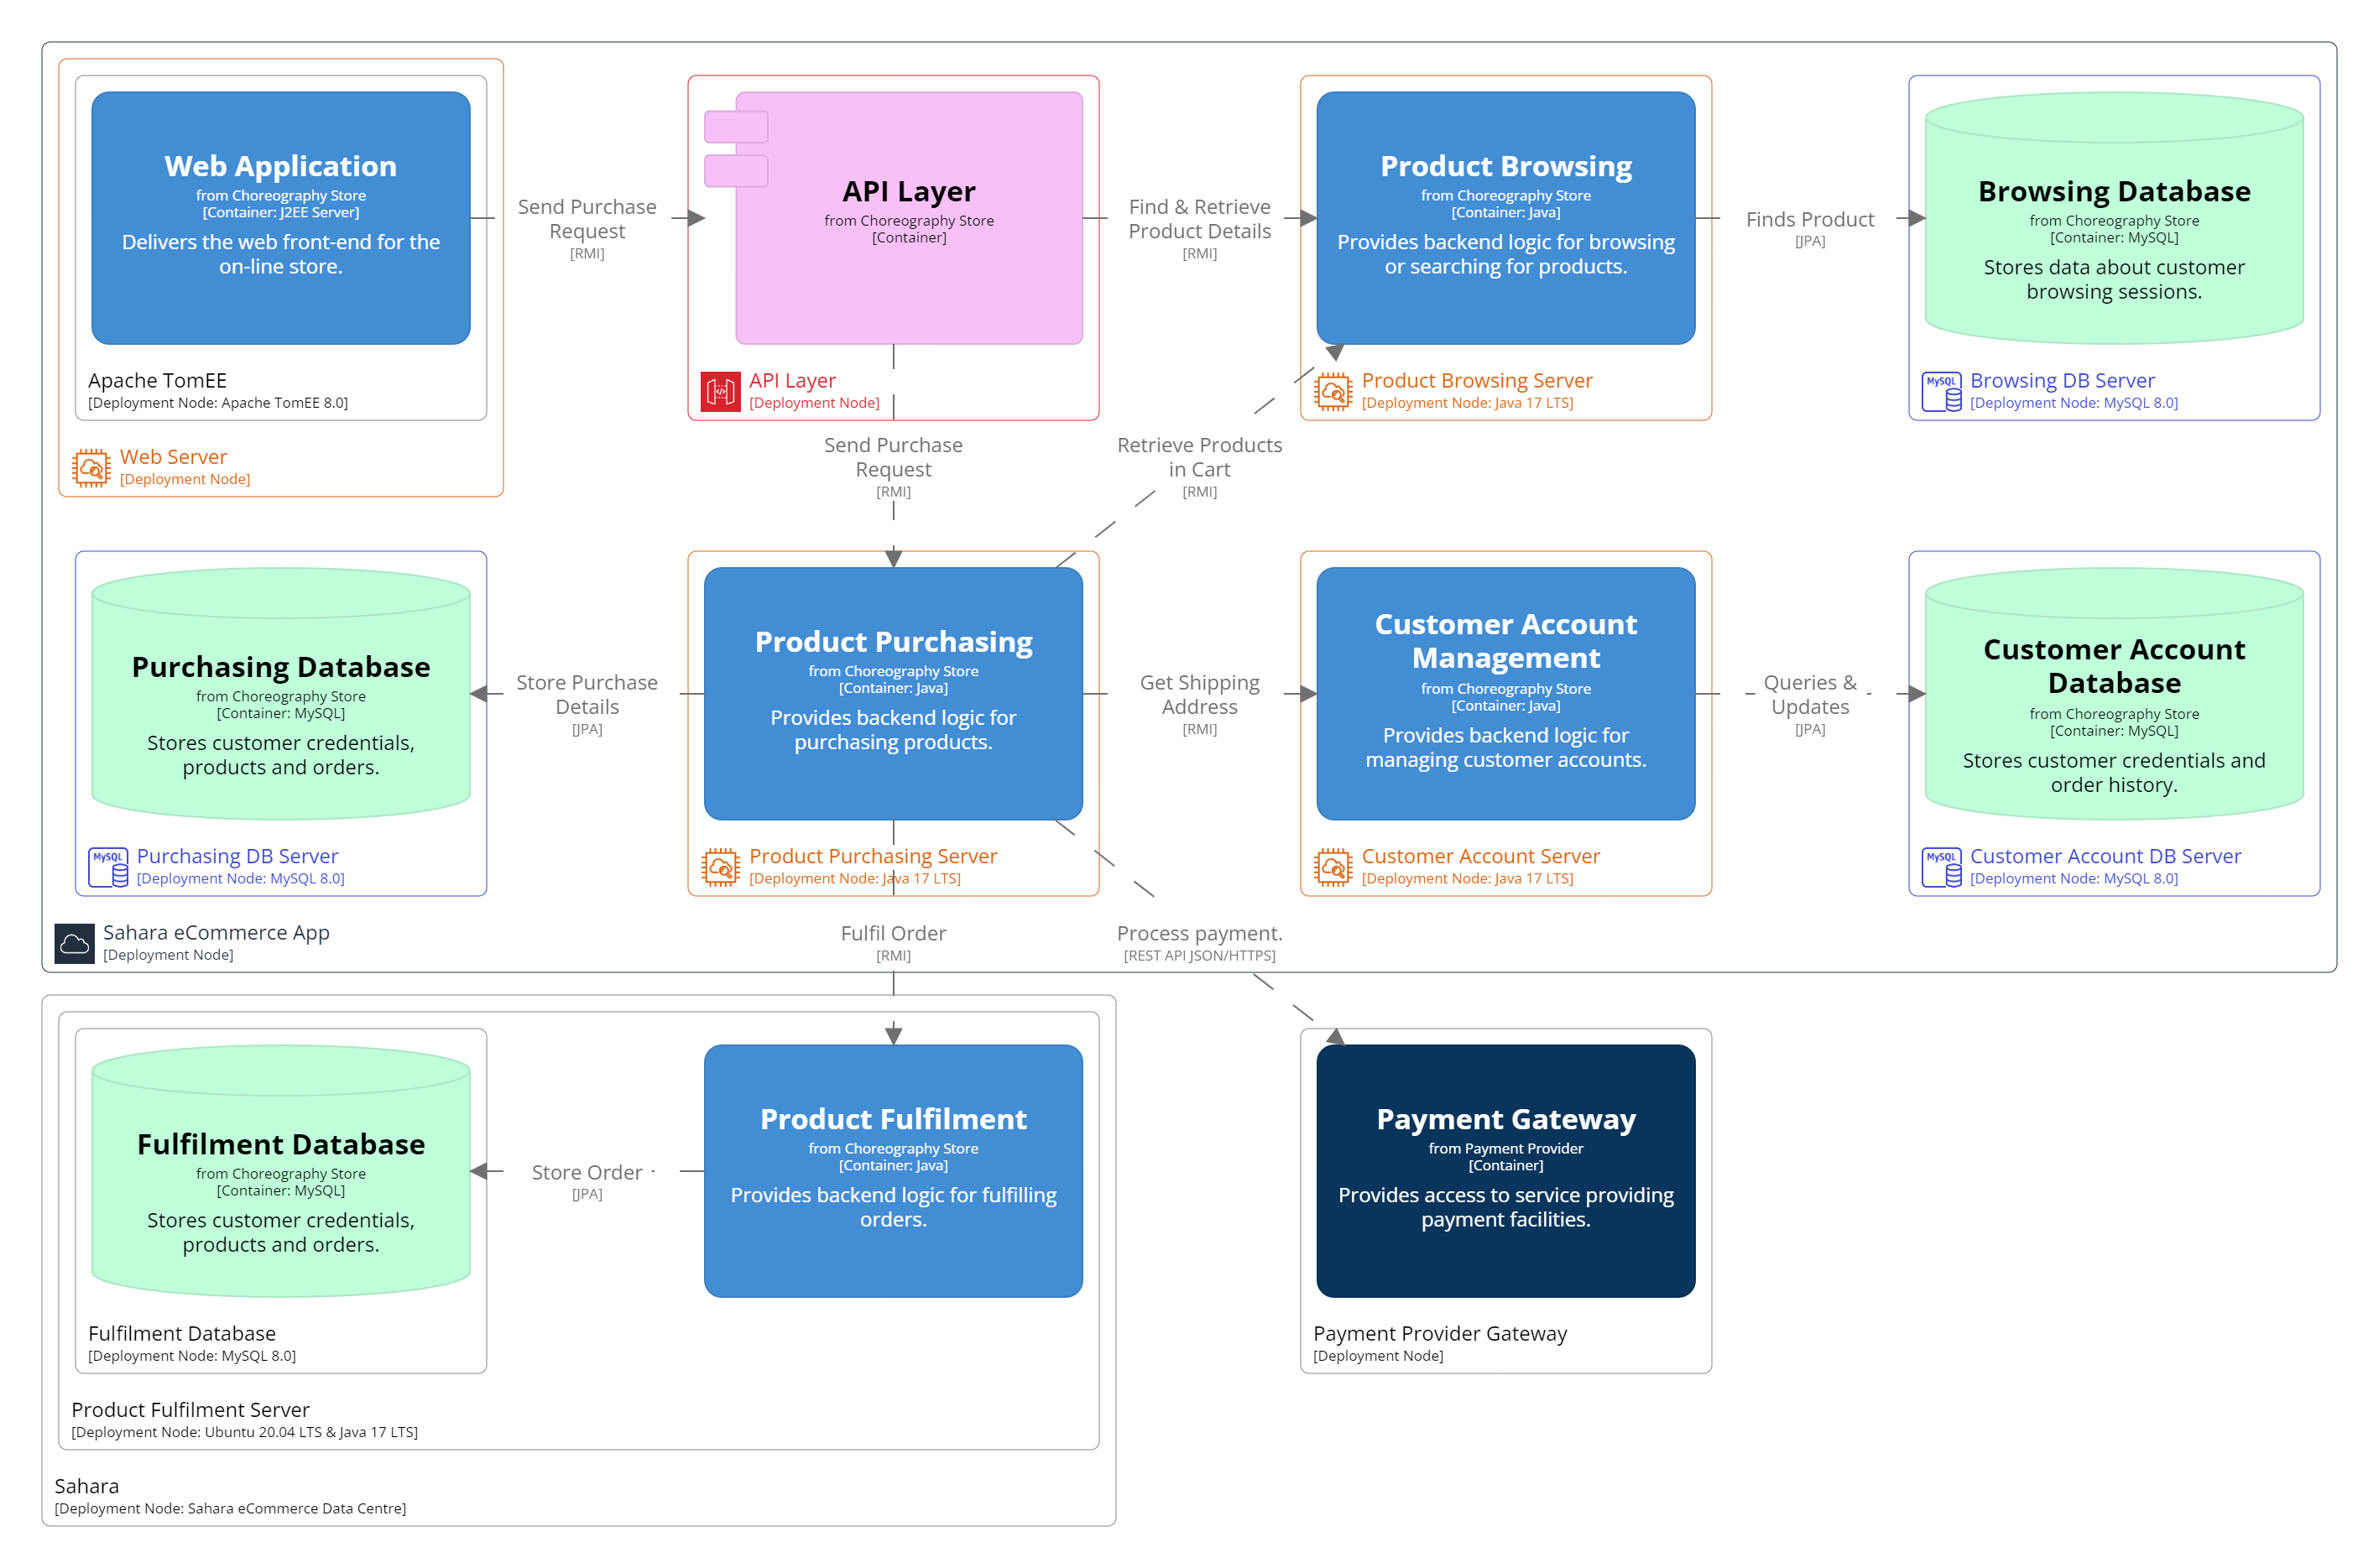
\includegraphics[trim=-80 45 45 40,clip,width=0.88\paperwidth]{diagrams/sahara-choreography-deployment.png}
    \end{adjustwidth}
	\begin{tikzpicture}[overlay,remember picture]
	\node[rectangle,shift={(0.9,1.4)},
		  text width=6cm,above,rotate=90] at (current page.west) {\color{primary}\Large Sahara using Choreography};
	\end{tikzpicture}   
\end{frame}

\begin{frame}{}
    \begin{adjustwidth}{-10mm}{-10mm}
        \centering
        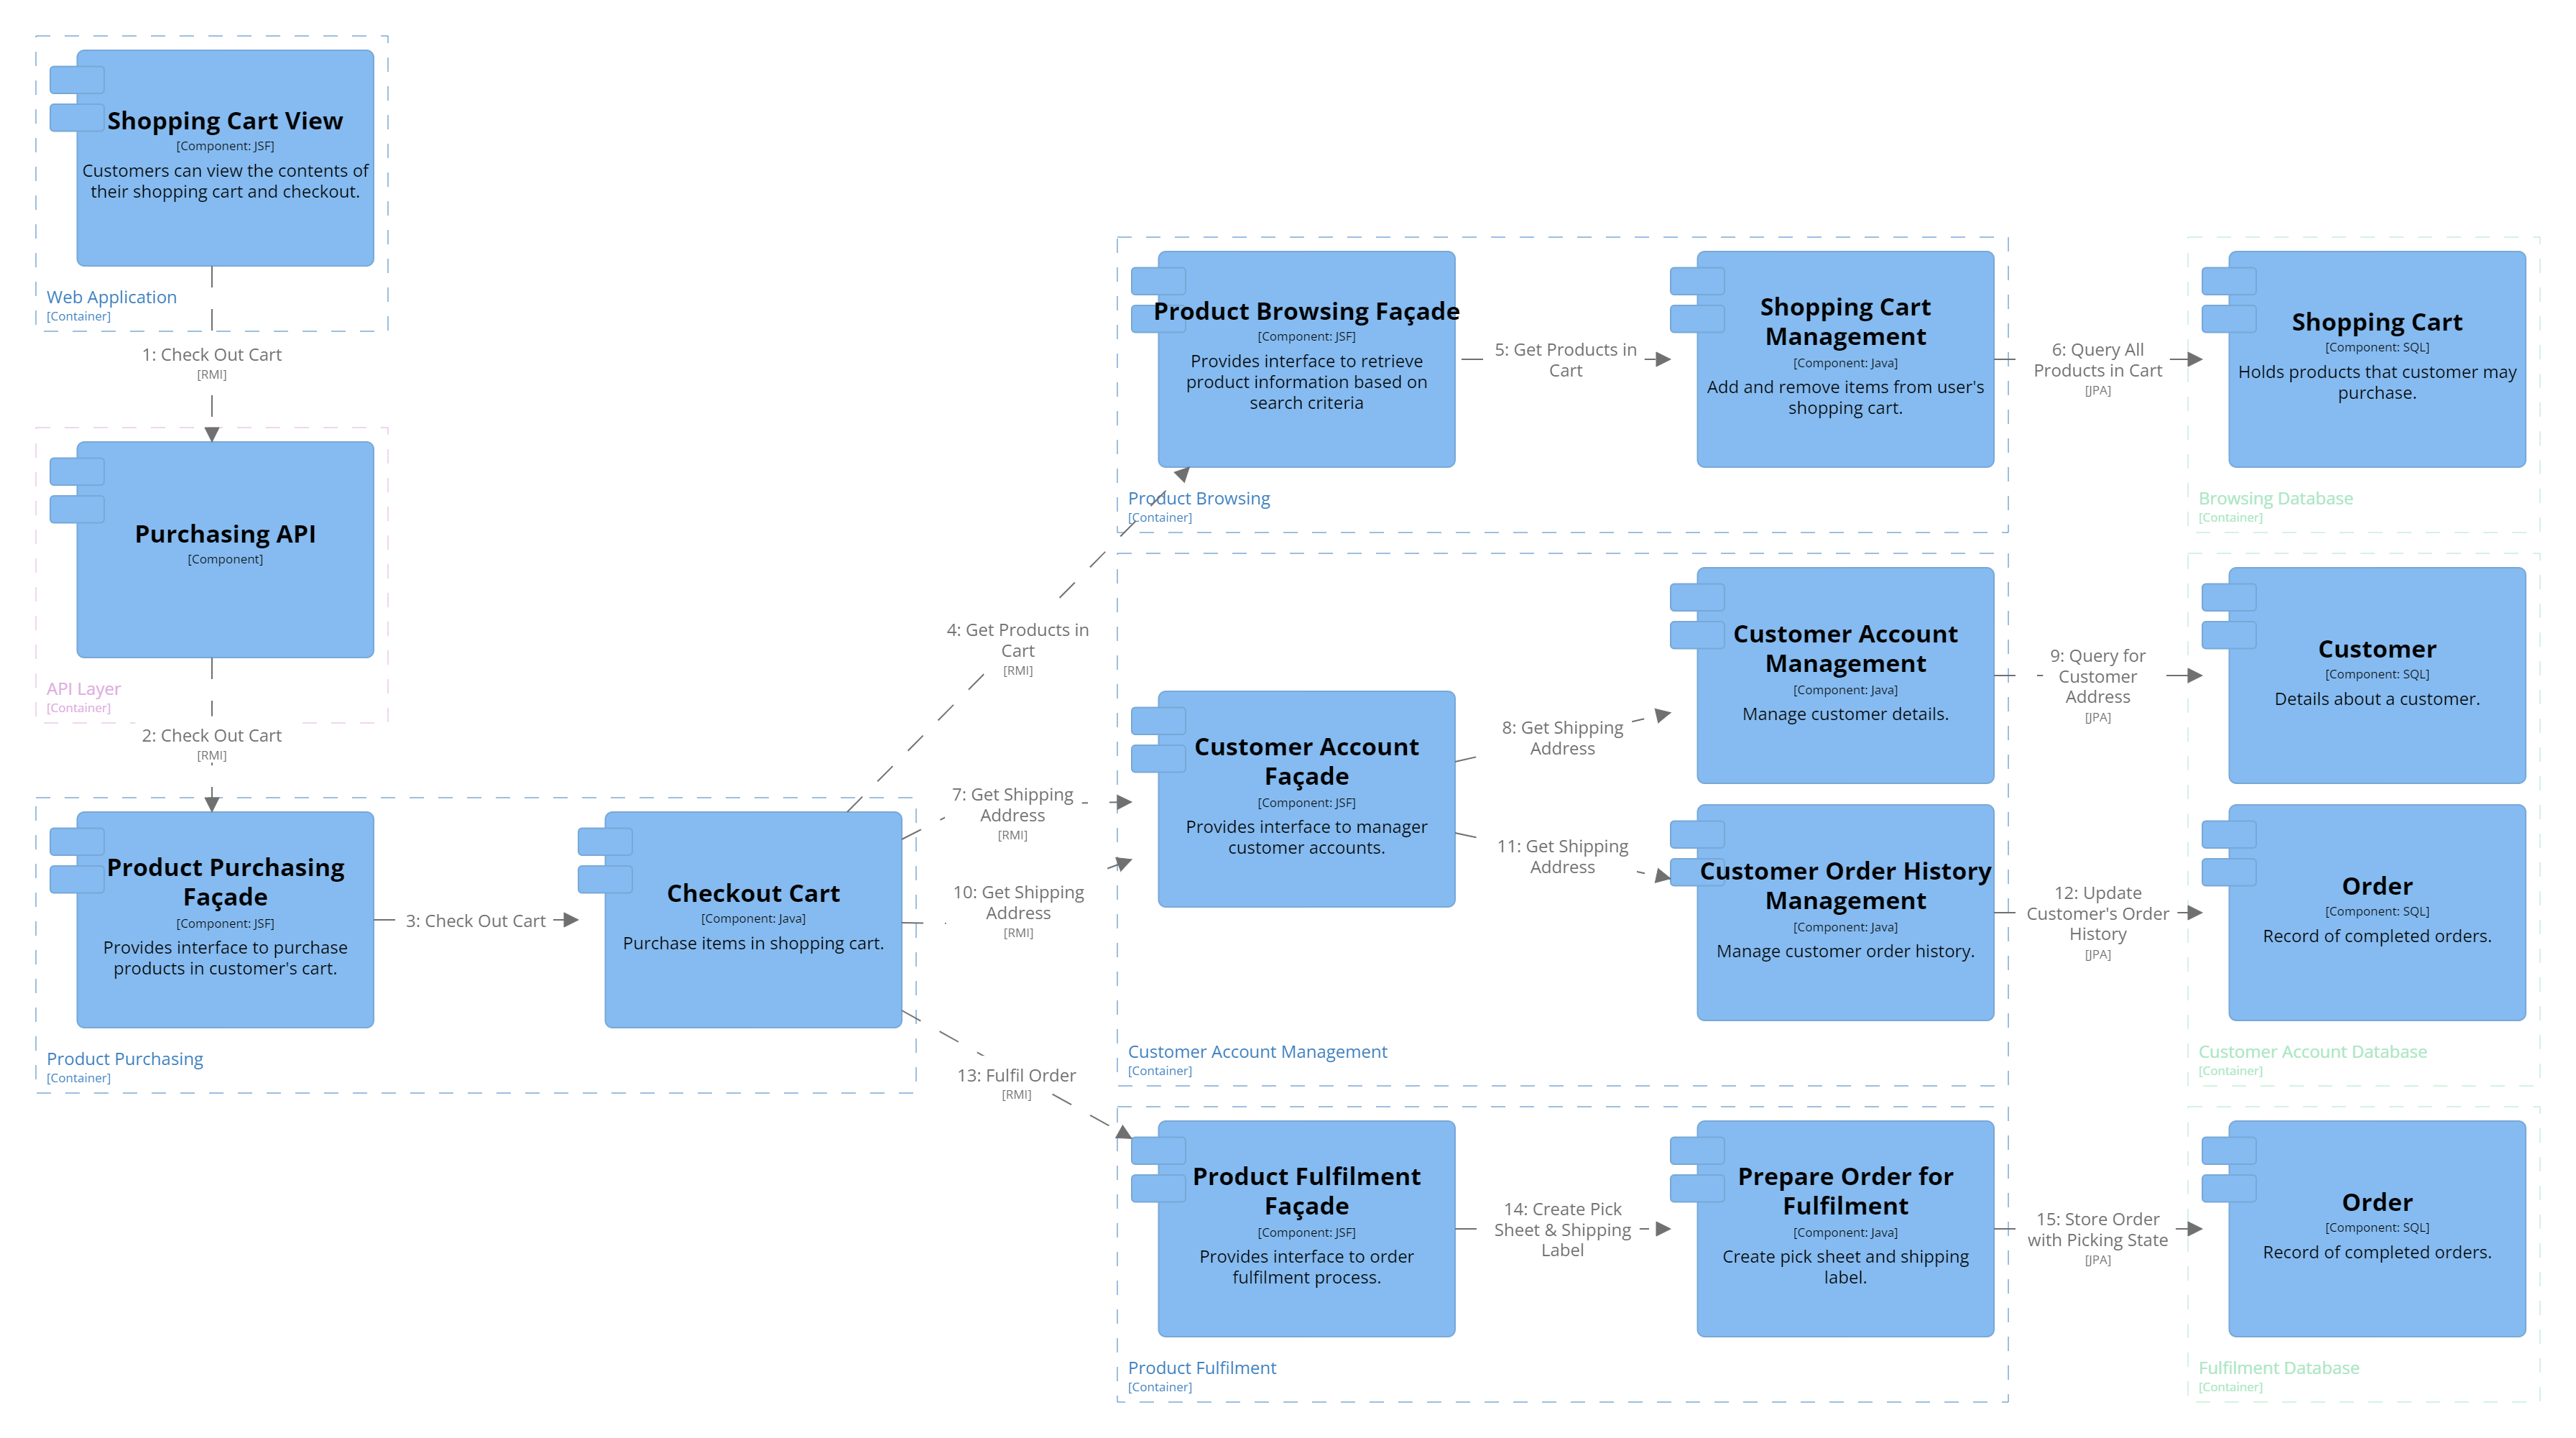
\includegraphics[trim=45 45 45 0,clip,width=0.98\paperwidth]{diagrams/sahara-choreography-purchase-products.png}
    \end{adjustwidth}
	\begin{tikzpicture}[overlay,remember picture]
	\node[rectangle,shift={(0.2,-0.9)},
		  text width=8cm,above] at (current page.north) {\color{primary}\Large Purchase Product Dynamic Diagram};
	\end{tikzpicture}   
\end{frame}

\begin{frame}
    \centering
    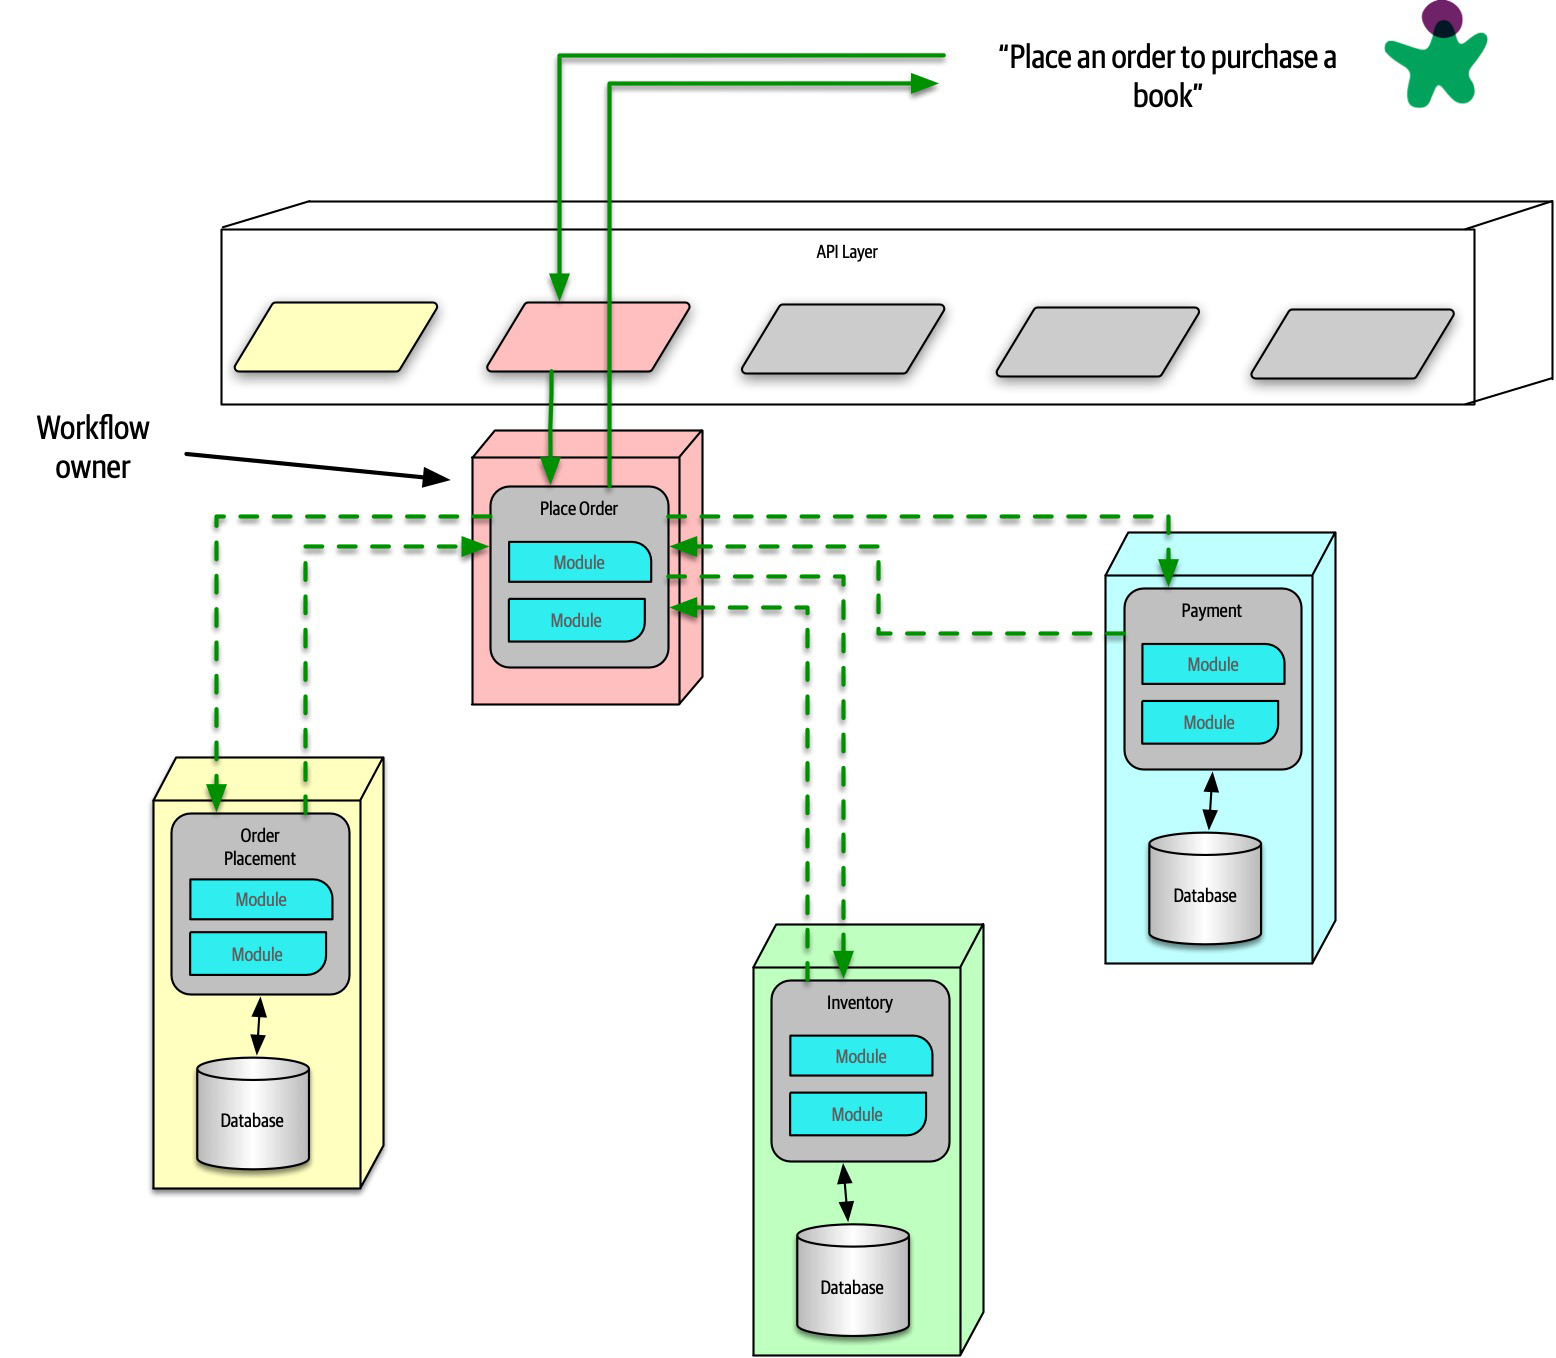
\includegraphics[height=.98\textheight]{diagrams/orchestration.png}
	\begin{tikzpicture}[overlay,remember picture]
	\node[rectangle,shift={(1.7,3.6)},
		  text width=3cm,above] at (current page.west) {\color{primary}\Large Orchestration};
	\end{tikzpicture}   
	\begin{tikzpicture}[overlay,remember picture]
	\node[rectangle,shift={(-4.6,0)},
		  text width=6.5cm,above] at (current page.south) {\color{primary}\tiny From \textit{Fundamentals of Software Architecture}};
	\end{tikzpicture}   
\end{frame}

\questionanswer{How bad is the coupling with choreography or orchestration?}
{For a large system, \highlight{very bad}.}
\note{In 2017, Uber had over 1400 services ... consider how bad coupling would be with either approach.}

\begin{frame}{}
	\centering
	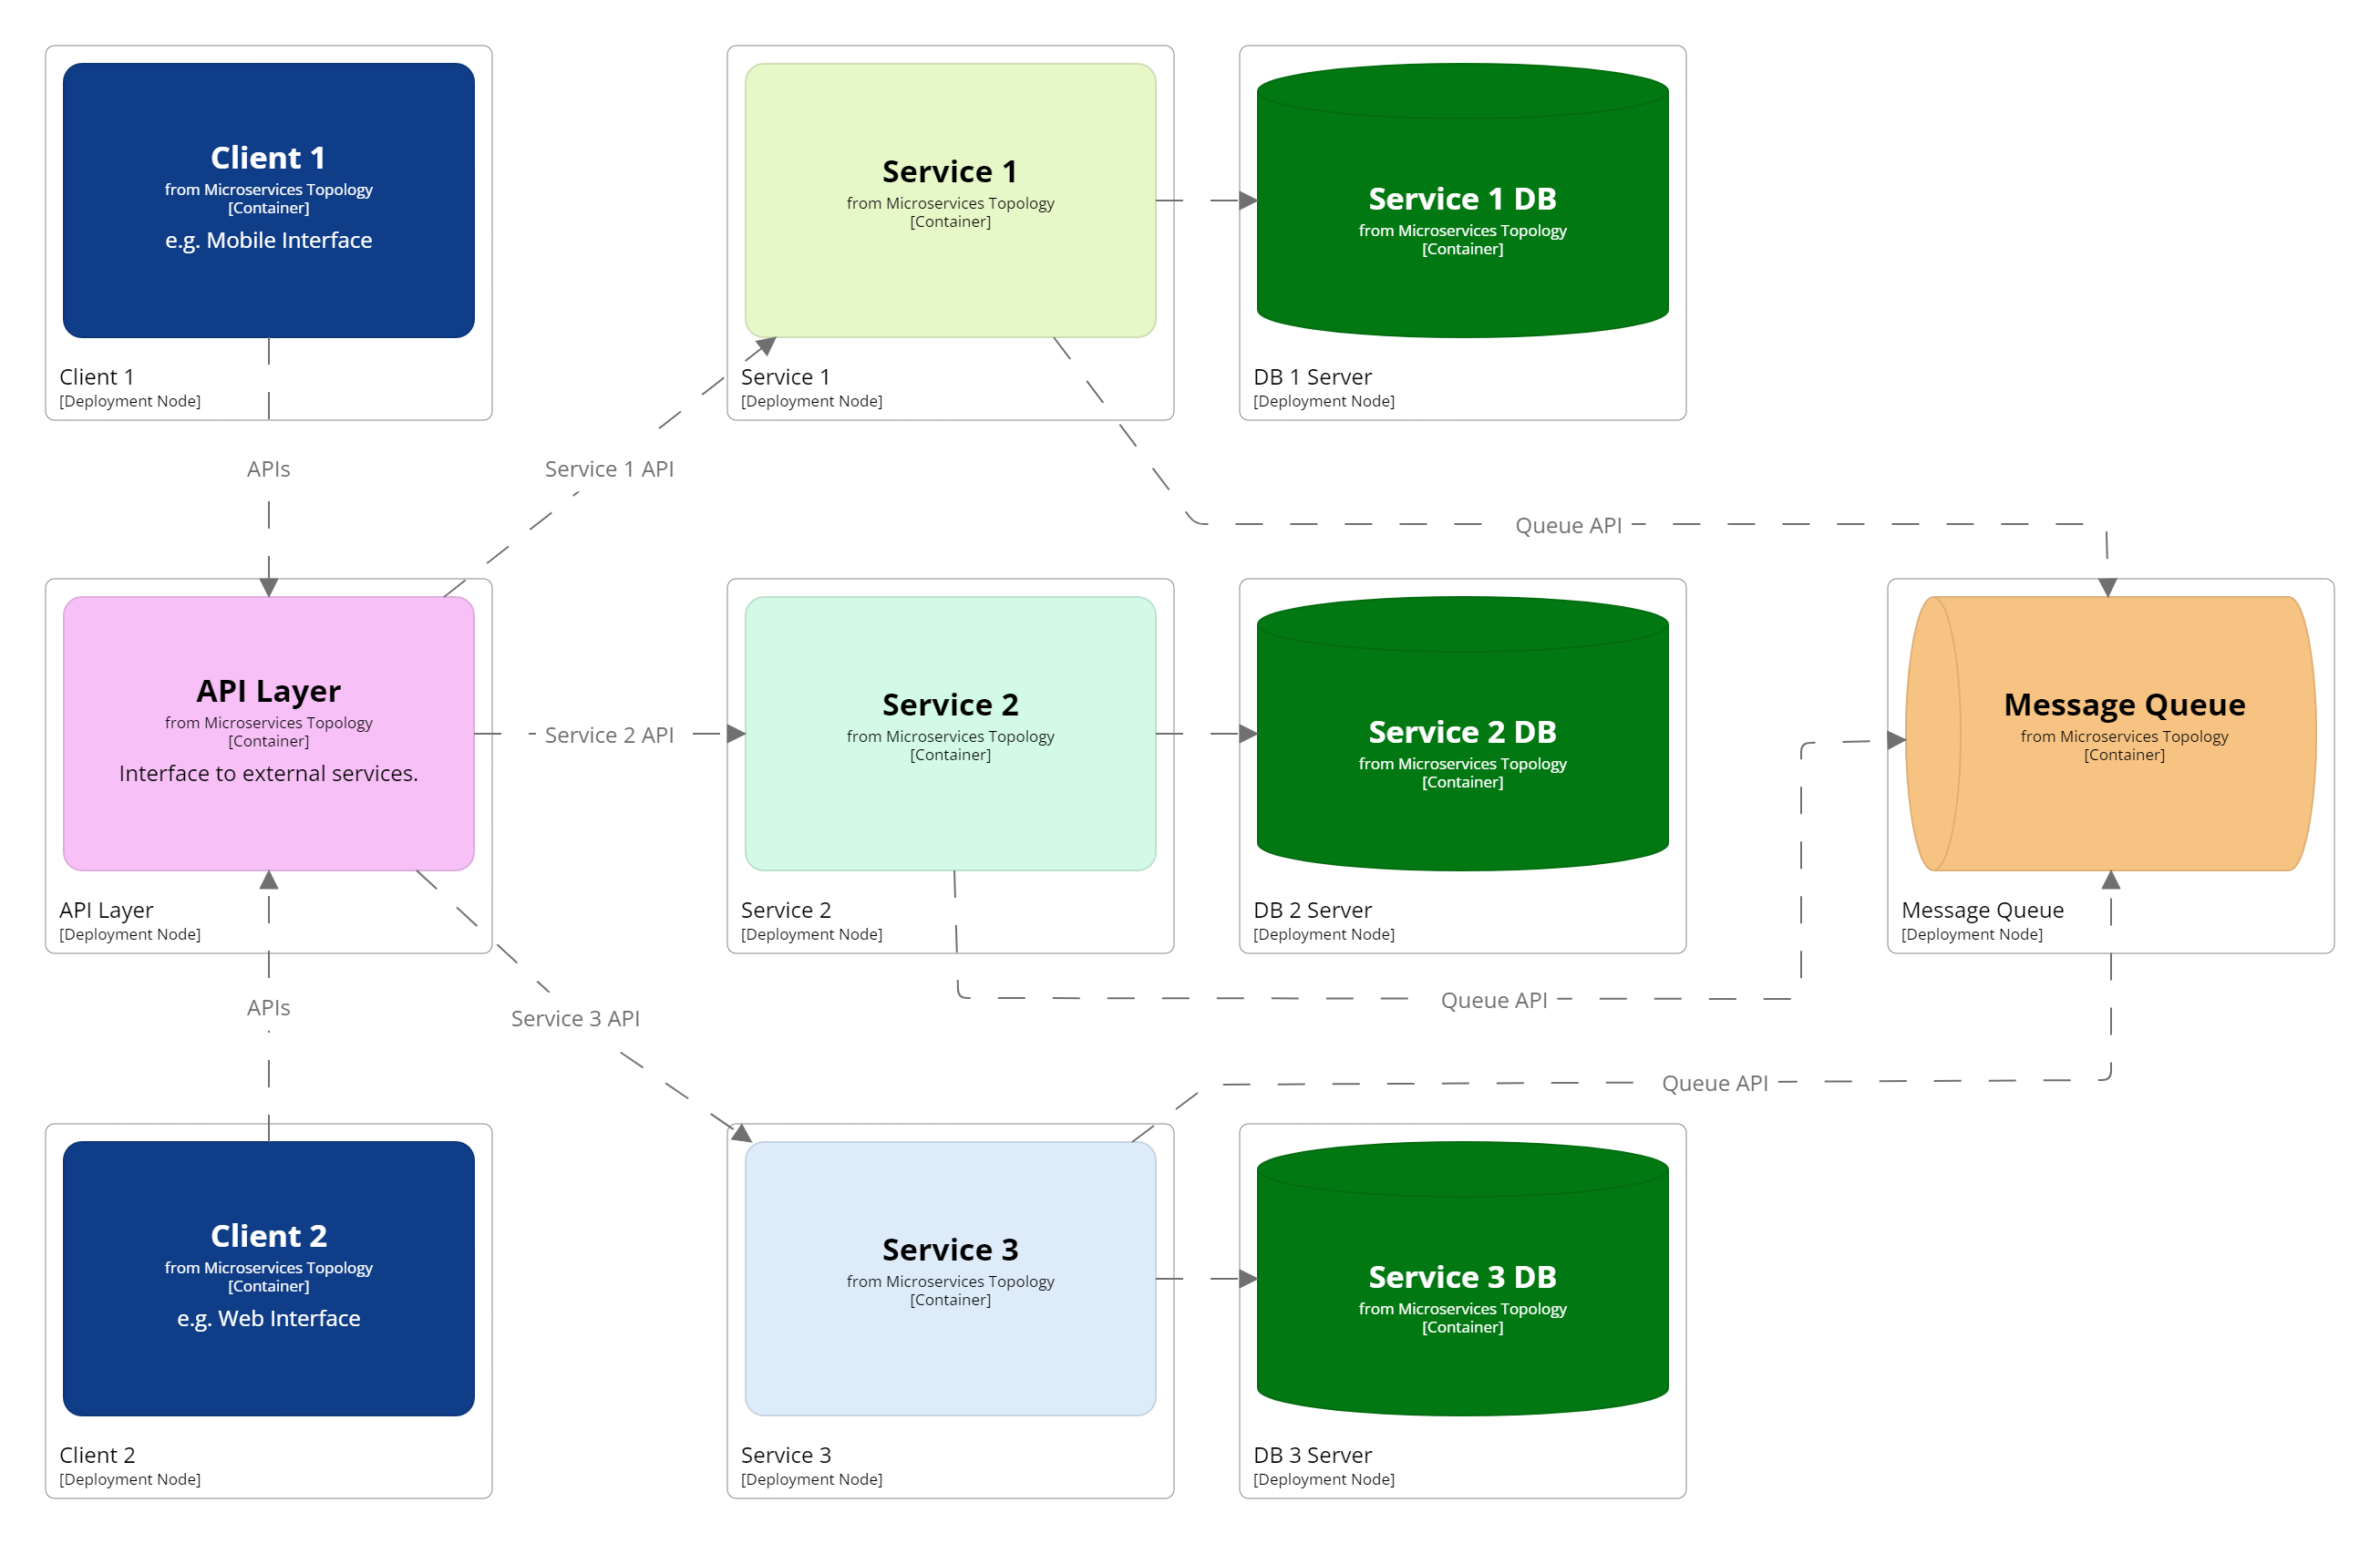
\includegraphics[trim=-50 45 45 45,clip,height=\textheight]{diagrams/event-queue-deployment.png}
	\begin{tikzpicture}[overlay,remember picture]
	\node[rectangle,shift={(0.9,0.8)},
		  text width=7cm,above,rotate=90] at (current page.west) {\color{primary}\Large Microservices with Event Queue};
	\end{tikzpicture}   
\end{frame}
\note[itemize]{
    \item Use the tried and true Observer pattern, with the event-driven architecture pattern.
    \item Services publish events indicating what they have been done.
    \item Services listen for events to decide how to coordinate their part of the system behaviour.
}

\begin{frame}{Service 1 Components with Event Queue}
    \begin{adjustwidth}{-10.5mm}{-10mm}
        \centering
        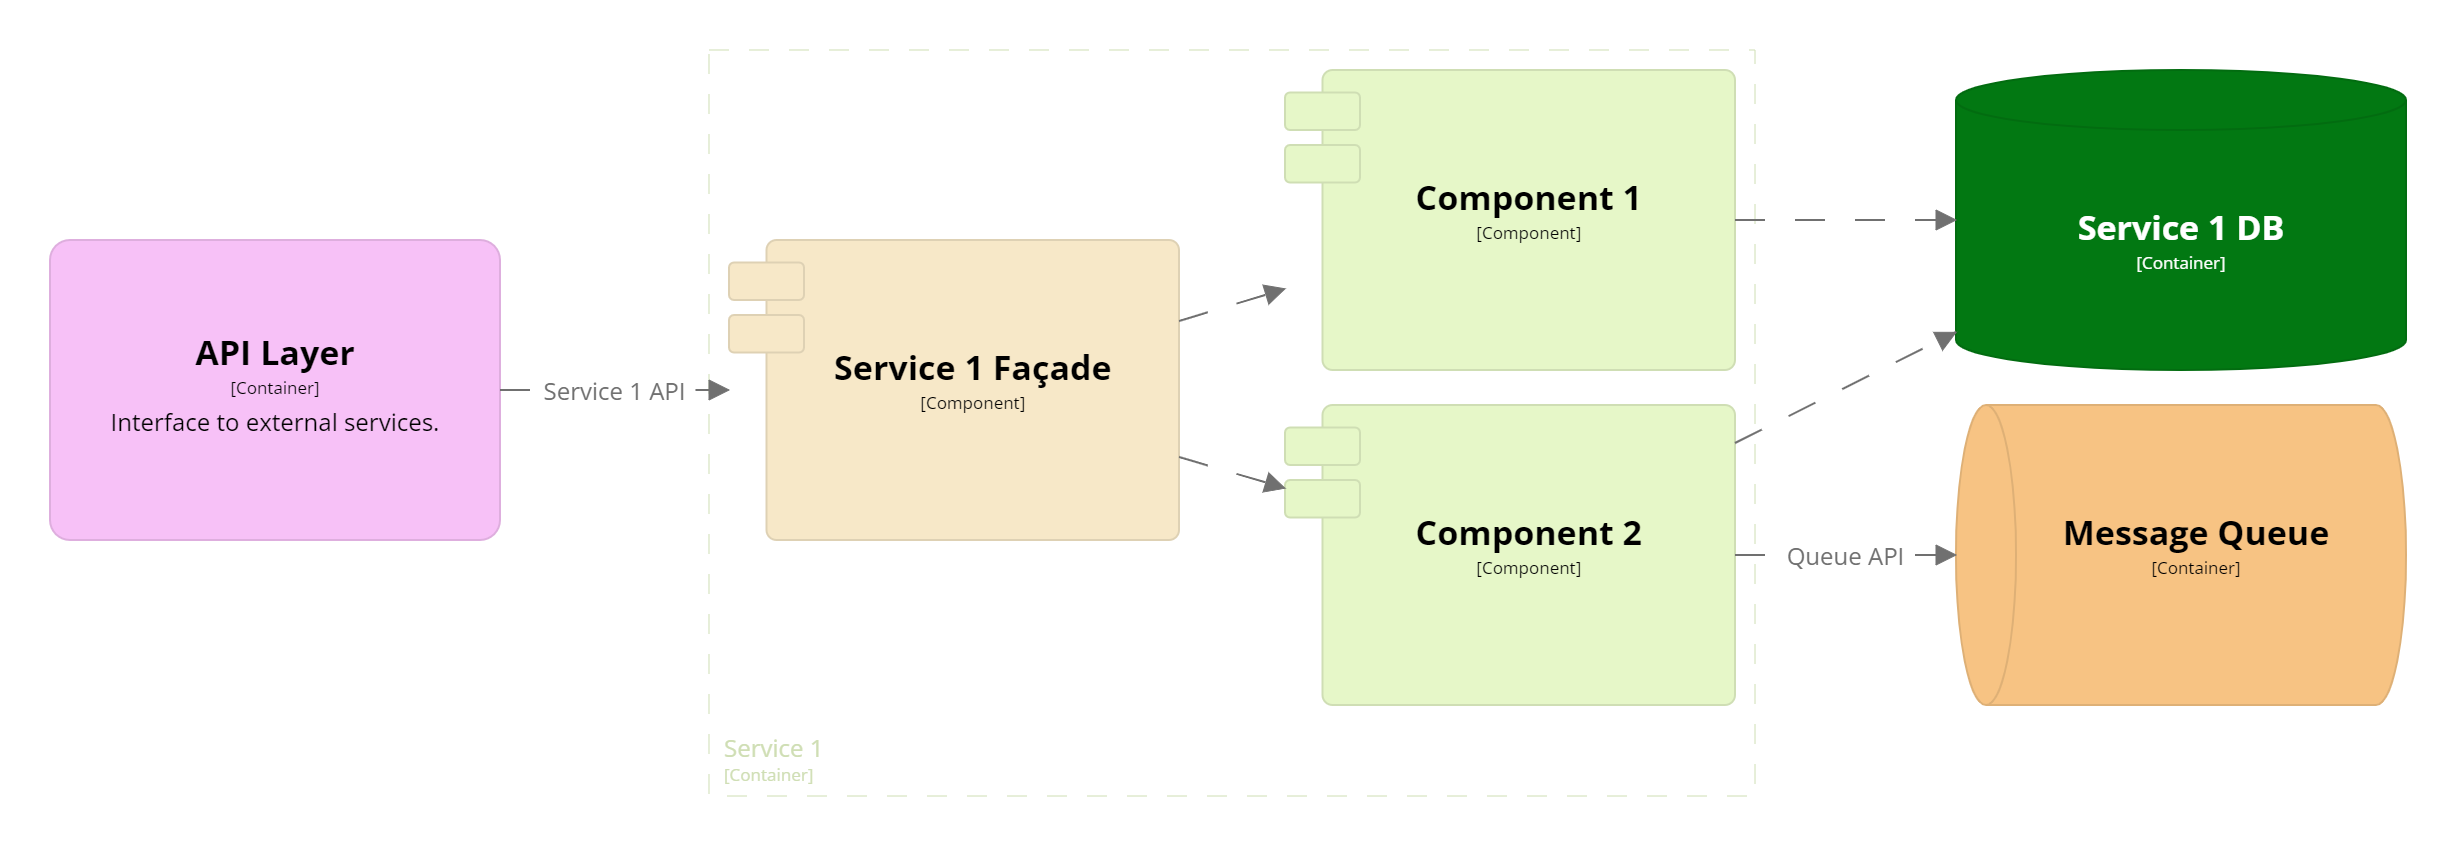
\includegraphics[trim=45 45 45 45,clip,width=0.99\paperwidth]{diagrams/event-queue-service1-component.png}
    \end{adjustwidth}
\end{frame}
\note{Services 2 \& 3 are essentially the same.}

\begin{frame}{}
    \begin{adjustwidth}{-10.5mm}{-10mm}
		\centering
		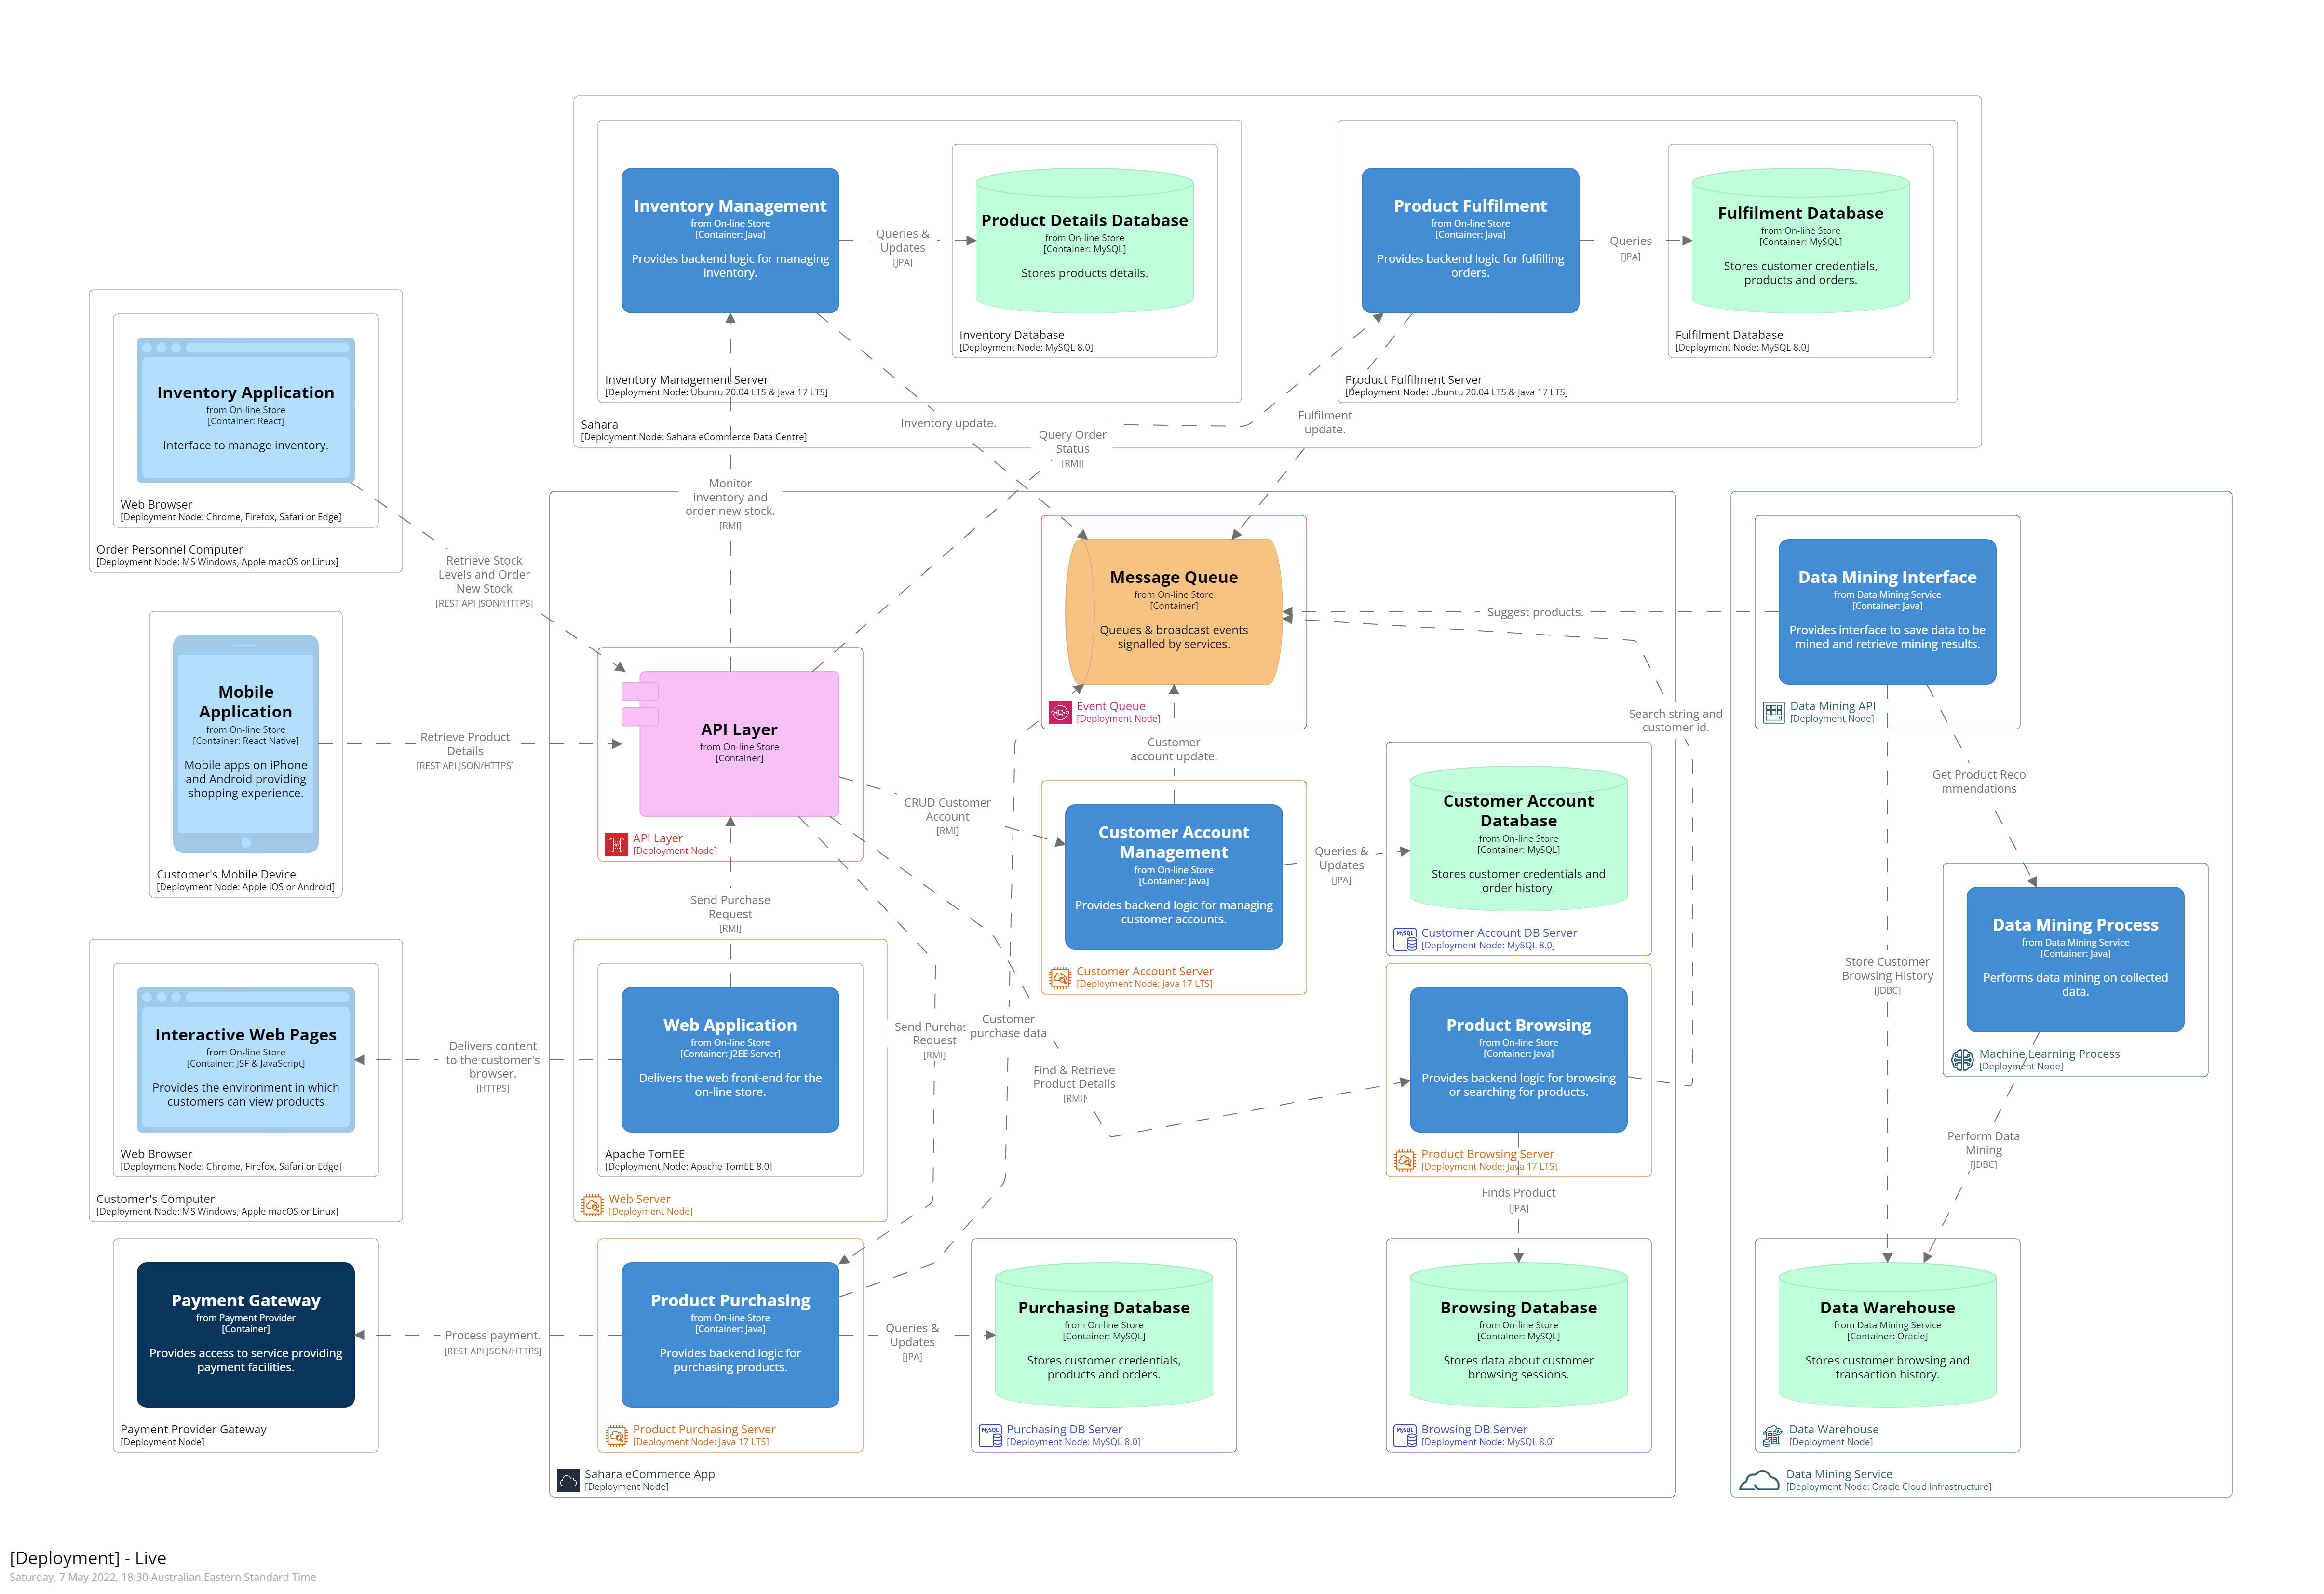
\includegraphics[trim=-130 160 140 195,clip,height=\textheight]{diagrams/sahara-microservices-1-deploy.png}
    \end{adjustwidth}
	\begin{tikzpicture}[overlay,remember picture]
	\node[rectangle,shift={(0.9,1.4)},
		  text width=7cm,above,rotate=90] at (current page.west) {\color{primary}\Large Sahara using an Event Queue};
	\end{tikzpicture}   
\end{frame}
\note[itemize]{
    \item Sahara eCommerce system as a simple microservices architecture, using event-driven messaging between services.
    \item Services publish events indicating what they have been done.
    \item Also an example of a multi-tenanted system built across in-house servers, AWS and OCI.
}

\questionanswer{Are \highlight{browsing} and \highlight{purchasing} separate contexts?}{
\begin{itemize}
    \item Are they a single business process or different processes?
    \item Do they share much or little data?
\end{itemize}
}
\note[itemize]{
    \item Probably different business processes, but possibly the same context.
    \item If separate services, browse needs to send an event for every change to the shopping cart, and purchase needs to listen for these.
    \item Possibly merge into one service, as one context.
}

\question{
\begin{itemize}
    \item What about \highlight{inventory management} and \highlight{browse}?
    \item How do they maintain a consistent product database?
\end{itemize}
}

\begin{frame}{Pros \& Cons}
    \vspace{1mm}
    {\LARGE
    \begin{description}
        \item[Modularity] \tabto{15em}
\includegraphics[width=8mm]{../../shared/images/thumbs-up.png}
        \item[Extensibility] \tabto{15em}
\includegraphics[width=8mm]{../../shared/images/thumbs-up.png}
        \item[Reliability] \tabto{15em}
\includegraphics[width=8mm]{../../shared/images/thumbs-up.png}
        \item[Interoperability] \tabto{15em}
\includegraphics[width=8mm]{../../shared/images/thumbs-up.png}
        \item[Scalability] \tabto{15em}
\includegraphics[width=8mm]{../../shared/images/thumbs-up.png}
        \item[Security] \tabto{15em}
\includegraphics[trim=57 145 70 85,clip,width=8mm]{../../shared/images/neutral.png}
        \item[Deployability] \tabto{15em}
\includegraphics[trim=22 19 22 12,clip,width=8mm]{../../shared/images/neutral.png}
        \item[Testability] \tabto{15em}
\includegraphics[trim=22 19 22 12,clip,width=8mm]{../../shared/images/neutral.png}
        \item[Simplicity] \tabto{15em}
\includegraphics[trim=22 19 22 12,clip,width=8mm]{../../shared/images/thumbs-down.png}
    \end{description}
    }
\end{frame}


%\bibliographystyle{ieeetr}
%\bibliography{books}

\end{document}